\def\year{2015}

%File: formatting-instruction.tex
\documentclass{IEEEtran}
%\documentclass[letterpaper]{article}
%usepackage{aaai}
\usepackage{times}
%\usepackage{helvet}
%\usepackage{courier}
\usepackage{cite}
\usepackage{graphicx}
\usepackage{url}
\usepackage{amsfonts}
\usepackage{moreverb}
%\usepackage{mathtools}
%%
%\usepackage{float}
\usepackage{bm}
\usepackage{paralist}
%\usepackage{minted}
%%
% so we don't need to specify figures subdirectory in figure code
%\graphicspath{{./figures/}}
\usepackage{subfig}
%\usepackage{minipage}
%needed to change table colors
\usepackage[table]{xcolor}
%\renewcommand{\arraystretch}{1.75} % General space between rows (1 standard)
%\renewcommand{\baselinestretch}{2}
\renewcommand\IEEEkeywordsname{Index Terms}
%%
%\frenchspacing
%\setlength{\pdfpagewidth}{8.5in}
%\setlength{\pdfpageheight}{11in}
%\pdfinfo{
%\title (Activity Monitoring and Prediction for Humans and NAO Humanoid Robots using Wearable Sensors)
%Author (Saminda Abeyruwan, Faisal Sikder, Ubbo Visser, Dilip Sarkar)}
%\setcounter{secnumdepth}{0}  
%\title{Semi-Automatic Extraction of  Training Examples from Sensor Readings for Activity Monitoring and Prediction for Humans and NAO Humanoid Robots}
\title{Semi-Automatic Extraction of  Training Examples from Sensor Readings for Activity Monitoring and Prediction for Humans}
%\title{Activity Monitoring and Prediction for Humans and NAO Humanoid Robots using 
%Wearable Sensors}
\author{{Saminda Abeyruwan}, {Dilip Sarkar}, {Faisal Sikder},   and {Ubbo Visser}
\thanks{ Authors are with
 the
Department of Computer Science, University of Miami,
  Coral Gables, FL, 33146, USA
{ emails:\{saminda, faisalsikder, visser, sarkar\}@cs.miami.edu};
\today} }
 \begin{document}
 %\begin{sloppy}
% The file aaai.sty is the style file for AAAI Press 
% proceedings, working notes, and technical reports.
\maketitle

\begin{abstract}
While humans or biped humanoid robots perform activities such as jogging and running, an accident 
event such as a fall may occur. This might cause damage to the human body or 
to the structural components of the robot. For humans, immediate identification of a fall 
will allow fast responses, while for a robot, early prediction can be used to take corrective 
measures to prevent a fall. Modern wireless sensing devices can be attached to humans or robots to 
collect motion data. We propose: \begin{inparaenum}[($i$)] \item 
methods to learn and predict different activities for humans and robots; and \item software 
tools to realize these functions  on embedded devices. \end{inparaenum} Our contributions include: 
\begin{inparaenum}[($i$)] \item detection of falls for both humans and robots within a unified 
framework; and \item  a  novel software development environment for embedded systems. 
\end{inparaenum} Our empirical evaluations demonstrate that with high accuracy different types of  
fall-events are predicted using the same learning algorithms for humans and biped humanoid robots. 
\end{abstract}

\begin{IEEEkeywords} Fall detection, learning algorithms, 9-axis sensor, semi-automatic extraction of training examples,  softmax, neural networks.
\end{IEEEkeywords}

%\tableofcontents

\section{Introduction}
\label{sec:Intro}
%Justification for activity monitoring
Fall is a major cause of injury to the elderly population \cite{Rubenstein2006}. 
Each year about 30-60\% of the elderly population have one or more falls, and  about 10-20\% of these falls results in injury \cite{Rubenstein2006}. 
As reported in CDC website \cite{CDC2014July},
``In 2010, falls among older adults cost the U.S. health care system \$30 billion in direct medical costs, when adjusted for inflation.'' By 2020 it is expected to reach \$67.7 billion. 
\par 
Availability of inexpensive miniature \emph{microelectromechanical system} (MEMS) sensors  has motivated researchers  to study their potential for assessing fall-risk  (see \cite{shanyReview2012}, \cite{howcroftReview2013}, and the references therein) as well as monitoring \emph{activities of daily livings} (ADLs) \cite{alvarezActivityAndFallRecognotion2015,BaoActivityrecognition2004,DernbachActivityAndFallDetectionPhone2012,krishnanActivityRecognition2014,kumarActivitAndFallDetection2013} and \emph{fall events} (FEs) \cite{baekFallDetection2013,baiFallDetectionPhone2013,DernbachActivityAndFallDetectionPhone2012,dumitracheFallDetection2013,kumarActivitAndFallDetection2013,leoneFallDetection2013,liangFallDetection2012,liFallDetection2009,moyaFallAndDamageDetection2015,ojetolaFallDetection2011,ShenFallDetectionPhone2015,steidlFallDetection2012,DoukasFallDetection2011,ErdoganFallDetection2014,JianFallDetection2015}. These studies have used  accelerometers,  or gyroscopes, or magnetometers, or  a combination of them to collect motion datasets at  25 Hz to 200 Hz.  
\par
Earlier studies demonstrated feasibility of various miniature wired or wireless devices, and recent studies have focused on extracting knowledge from motion sensor data.  Results from past studies have proven  that hardware for MEMS sensor based \emph{intelligent} devices to \begin{inparaenum} [($i$)] \item assess fall-risks, \item monitor ADLs, and \item identify fall events have reached maturity and can be assembled from off-the-shelf hardware. \end{inparaenum}  

\par
Remaining major challenges include automatic development of \begin{inparaenum}[($i$)] \item firmware and software for collecting motion data and  extracting features specific to applications and users, and \item software module for making intelligent decisions utilizing features extracted from motion data. \end{inparaenum}
For example, a device with 9-axis MEMS motion sensor to be used for identifying four fall events --- fall forward, fall backward, fall left, and fall right. The device must have firmware modules to collect motion data, to preprocess motion data, and to extract sufficient features from the preprocessed data for identification of all fall events. Also, the device must have a software module that takes the extracted features as input and recognizes correctly  which fall event has occurred.

%However, the challenges: How to gather \textbf{\emph{sufficient }} motion datasets and how to \emph{\textbf{automate }} extraction of required information form the datasets  for assessment of fall-risks.

%The humans as well as the biped humanoid robots performs similar activities --- such as, jogging, and running etc. While performing these routine 
%activities, accidents such as falls may occur causing damage to the human body or to the structural 
%components of the humanoid robot \cite{moyaFallAndDamageDetection2015}. 
%In the near future human-robot will cooperatively work together for solving problems that are difficult for both groups.  For instance, there has been an increasing demand in 
%domains such as rescue to use autonomous or teleoperated humanoid robots to complete high-risk 
%tasks, otherwise would have been lethal to a human subject. Therefore, we envision environments 
%where humans and humanoid robots collaboratively work to complete tasks. 
\par
Since both humans and biped humanoid robots have almost identical movements and are susceptible to 
similar accidents, we believe that the same devices are suitable for monitoring activities and fall events of both 
groups. Moreover, in the near future human-robot will cooperatively work together for solving problems that are impossible for either group but can be done with a combination of both groups.  For instance, there has been an increasing demand in 
domains such as rescue to use autonomous or teleoperated humanoid robots to complete high-risk 
tasks, otherwise would have been lethal to a human subject. Therefore, we envision environments 
where humans and humanoid robots collaboratively work to complete tasks. 

\par
To validate our hypotheses, we developed a generalized approach for learning 
and predicting activities of both groups \cite{abeyruwanFlairs2015}.  We attached wearable sensing devices to collect
motion data and have used software tools to interpret the sensor data to distinguish 
between regular activities and fall events (see Fig.~\ref{fig:deviceWithSubjects}). 
In our study, all four fall and seven non-fall activities of biped robots were identified with 100\%  accuracy after using Kalman filter \cite{Welch:1995:IKF:897831} with appropriate thresholding. However, for the same set of activities of human subjects, we could not use \emph{Kalman filtering} technique, because datasets for human subject had too much availabilities. And using Logistic Regression and \emph{Support Vector Machines} (SVM) true positive recognition was low as 90\%. The most \emph{ad hoc} and arduous part of our work was extraction of training datasets from the time series, which was part of the motivation for the work presented in this paper.
% to investigate the prospect of using external embedded 
%devices to identify activities on a NAO humanoid robot. 

%\par
%In this work, we concentrate on extracting training datasets and test datasets from time-series collected from the device. For each type of activity to be monitored we collect nine time-series using a 9-axis MEMS sensor.  
%
%Before we report our contributions, we provide a brief review of work related to identification of 
%human activity.  



%  The microcontrollers and embedded devices provide a flexible platform to build may 
% real world applications. In order to build these applications, a practitioner would require  
% flexible and reliable software solutions. A practitioner also may require to use more than one 
% functionality provided by the devices to build applications. Existing software solutions provide 
% facilities to build applications to a certain degree, but, they lack methods or systems to 
% integrate 
% multiple devices simultaneously without much user burden. We have developed  a state-of-the-art 
% open 
% source software solution to build heterogeneous applications on many devices, which can be 
% programmed on multiple operating systems. 
%%%% Commented below is the version in FLAIRS
%\begin{figure*}[!t]
%\centering
%\begin{minipage}{0.84\textwidth}
%\subfloat[]{\label{fig:fa}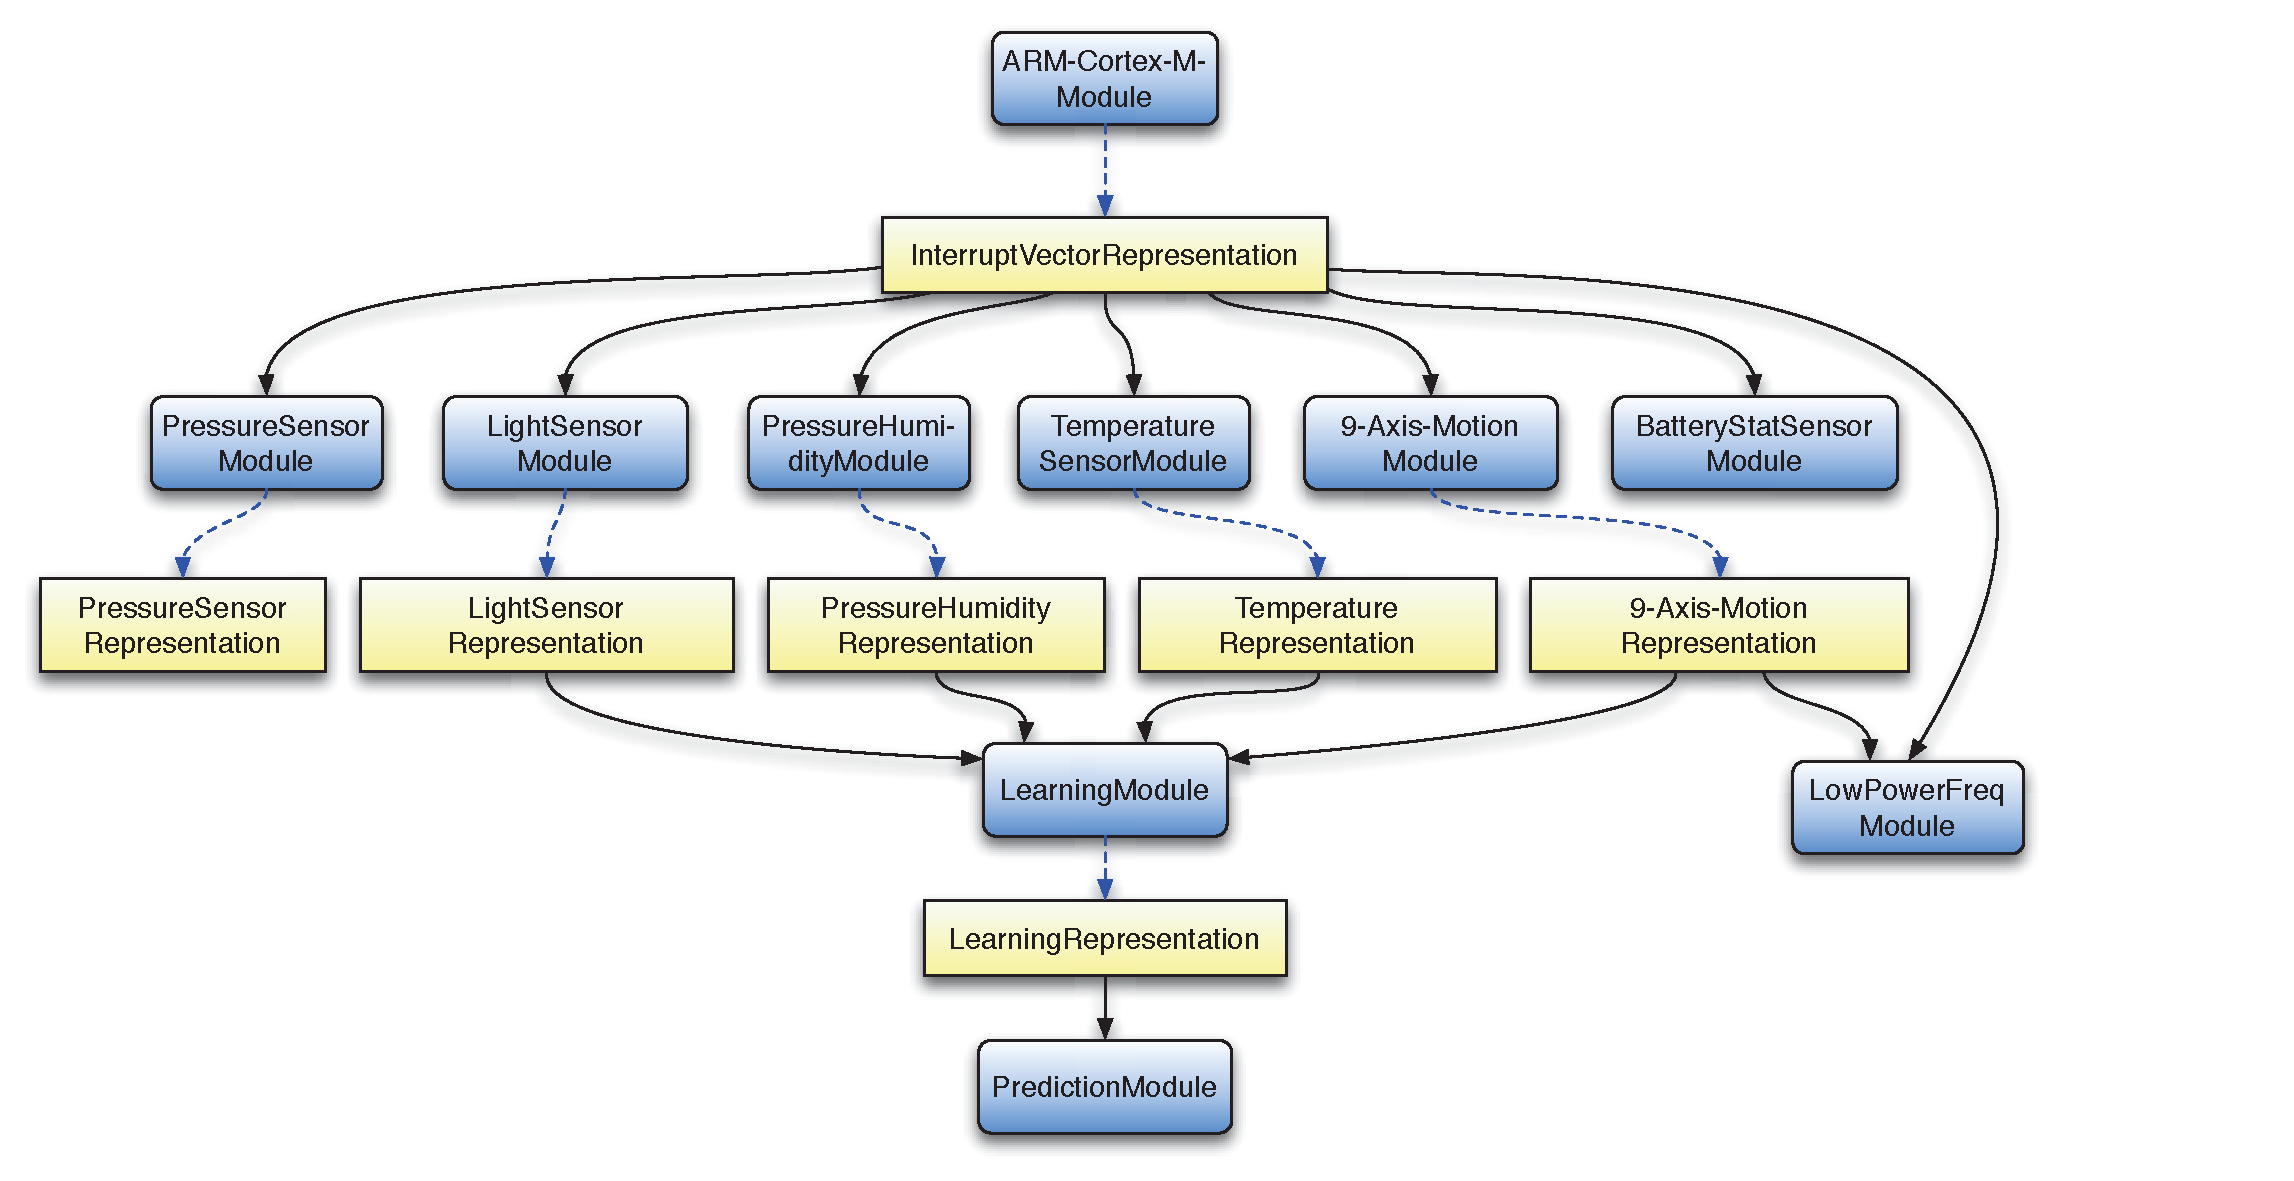
\includegraphics[width=\textwidth,height=3.5in]{figures/graph_structure_def-crop3.eps}}
%\end{minipage}
%\begin{minipage}{.12\textwidth}
%\begin{subfigure}
%\subfloat[]{\label{fig:fb}\includegraphics[width=\textwidth]{figures/human_figure.eps}}
%\end{subfigure}
%\begin{subfigure}
%\subfloat[]{\label{fig:fc}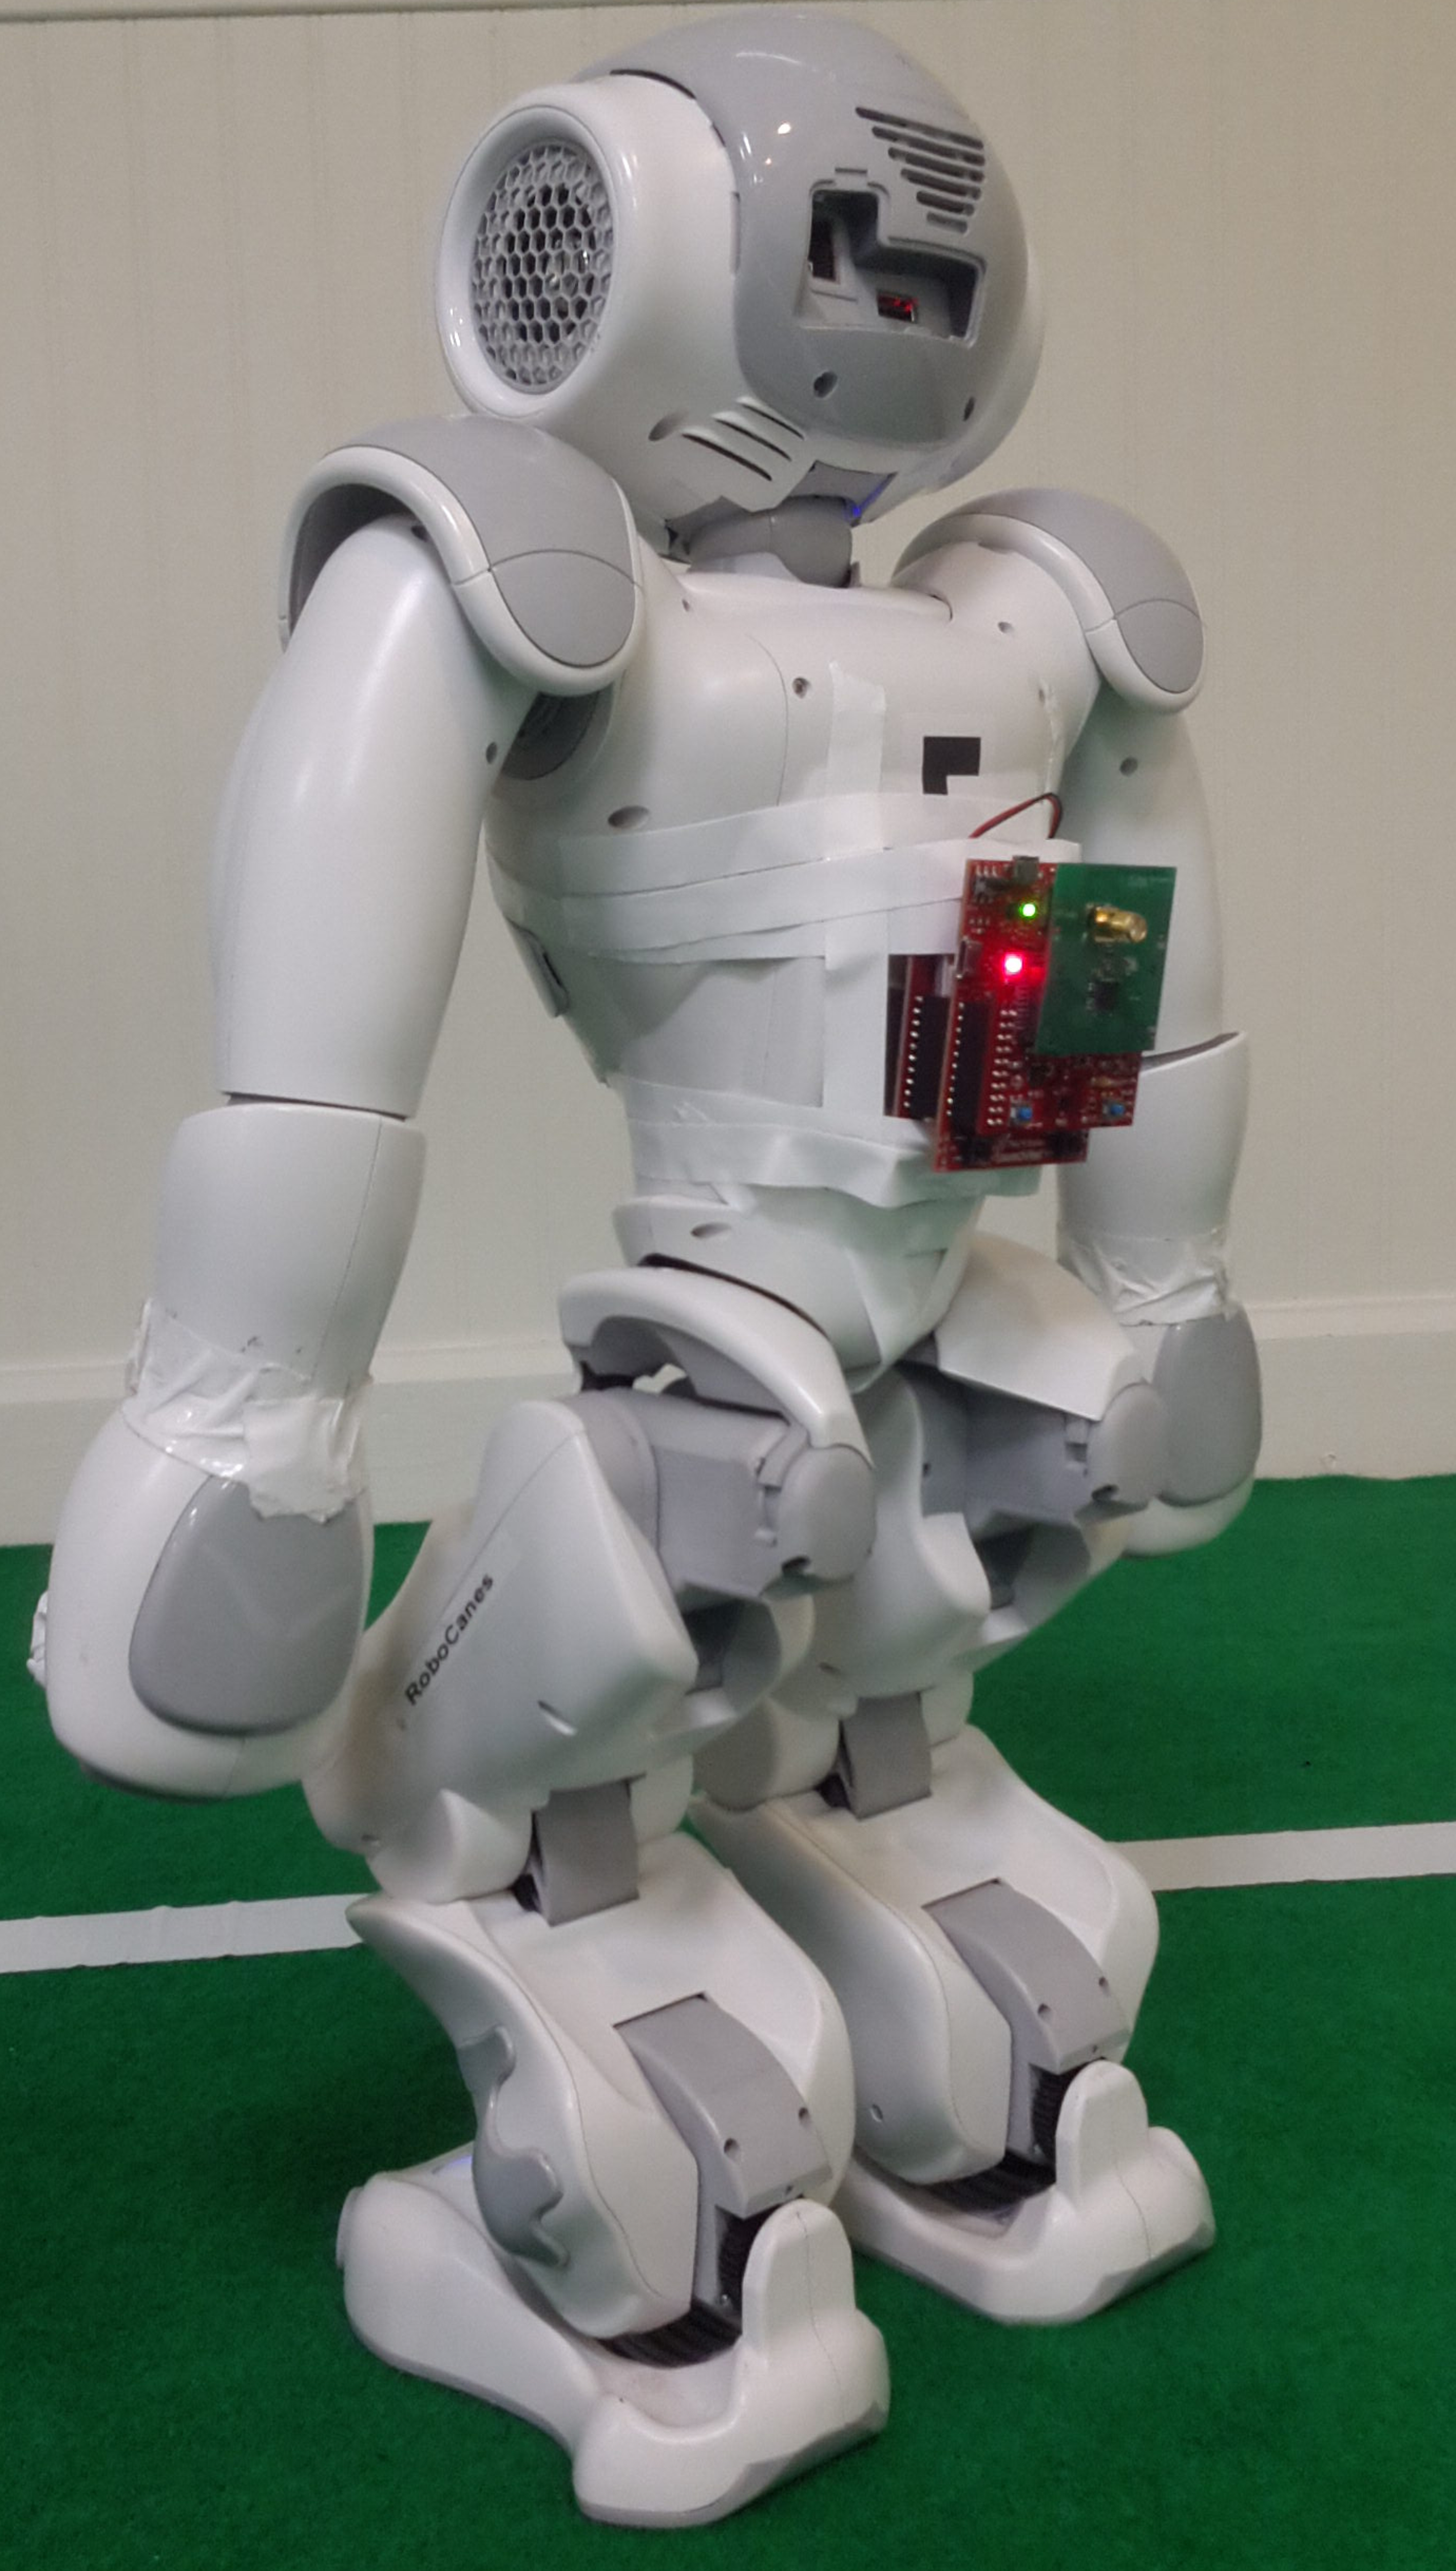
\includegraphics[width=\textwidth]{figures/robot_figure.eps}} 
%\end{subfigure}
%\end{minipage}


\begin{figure}[htb]
\centering
\subfloat[]{\label{fig:fb}\includegraphics[width=0.45\columnwidth]{figures/human_figure.eps}}
\qquad
\subfloat[]{\label{fig:fc}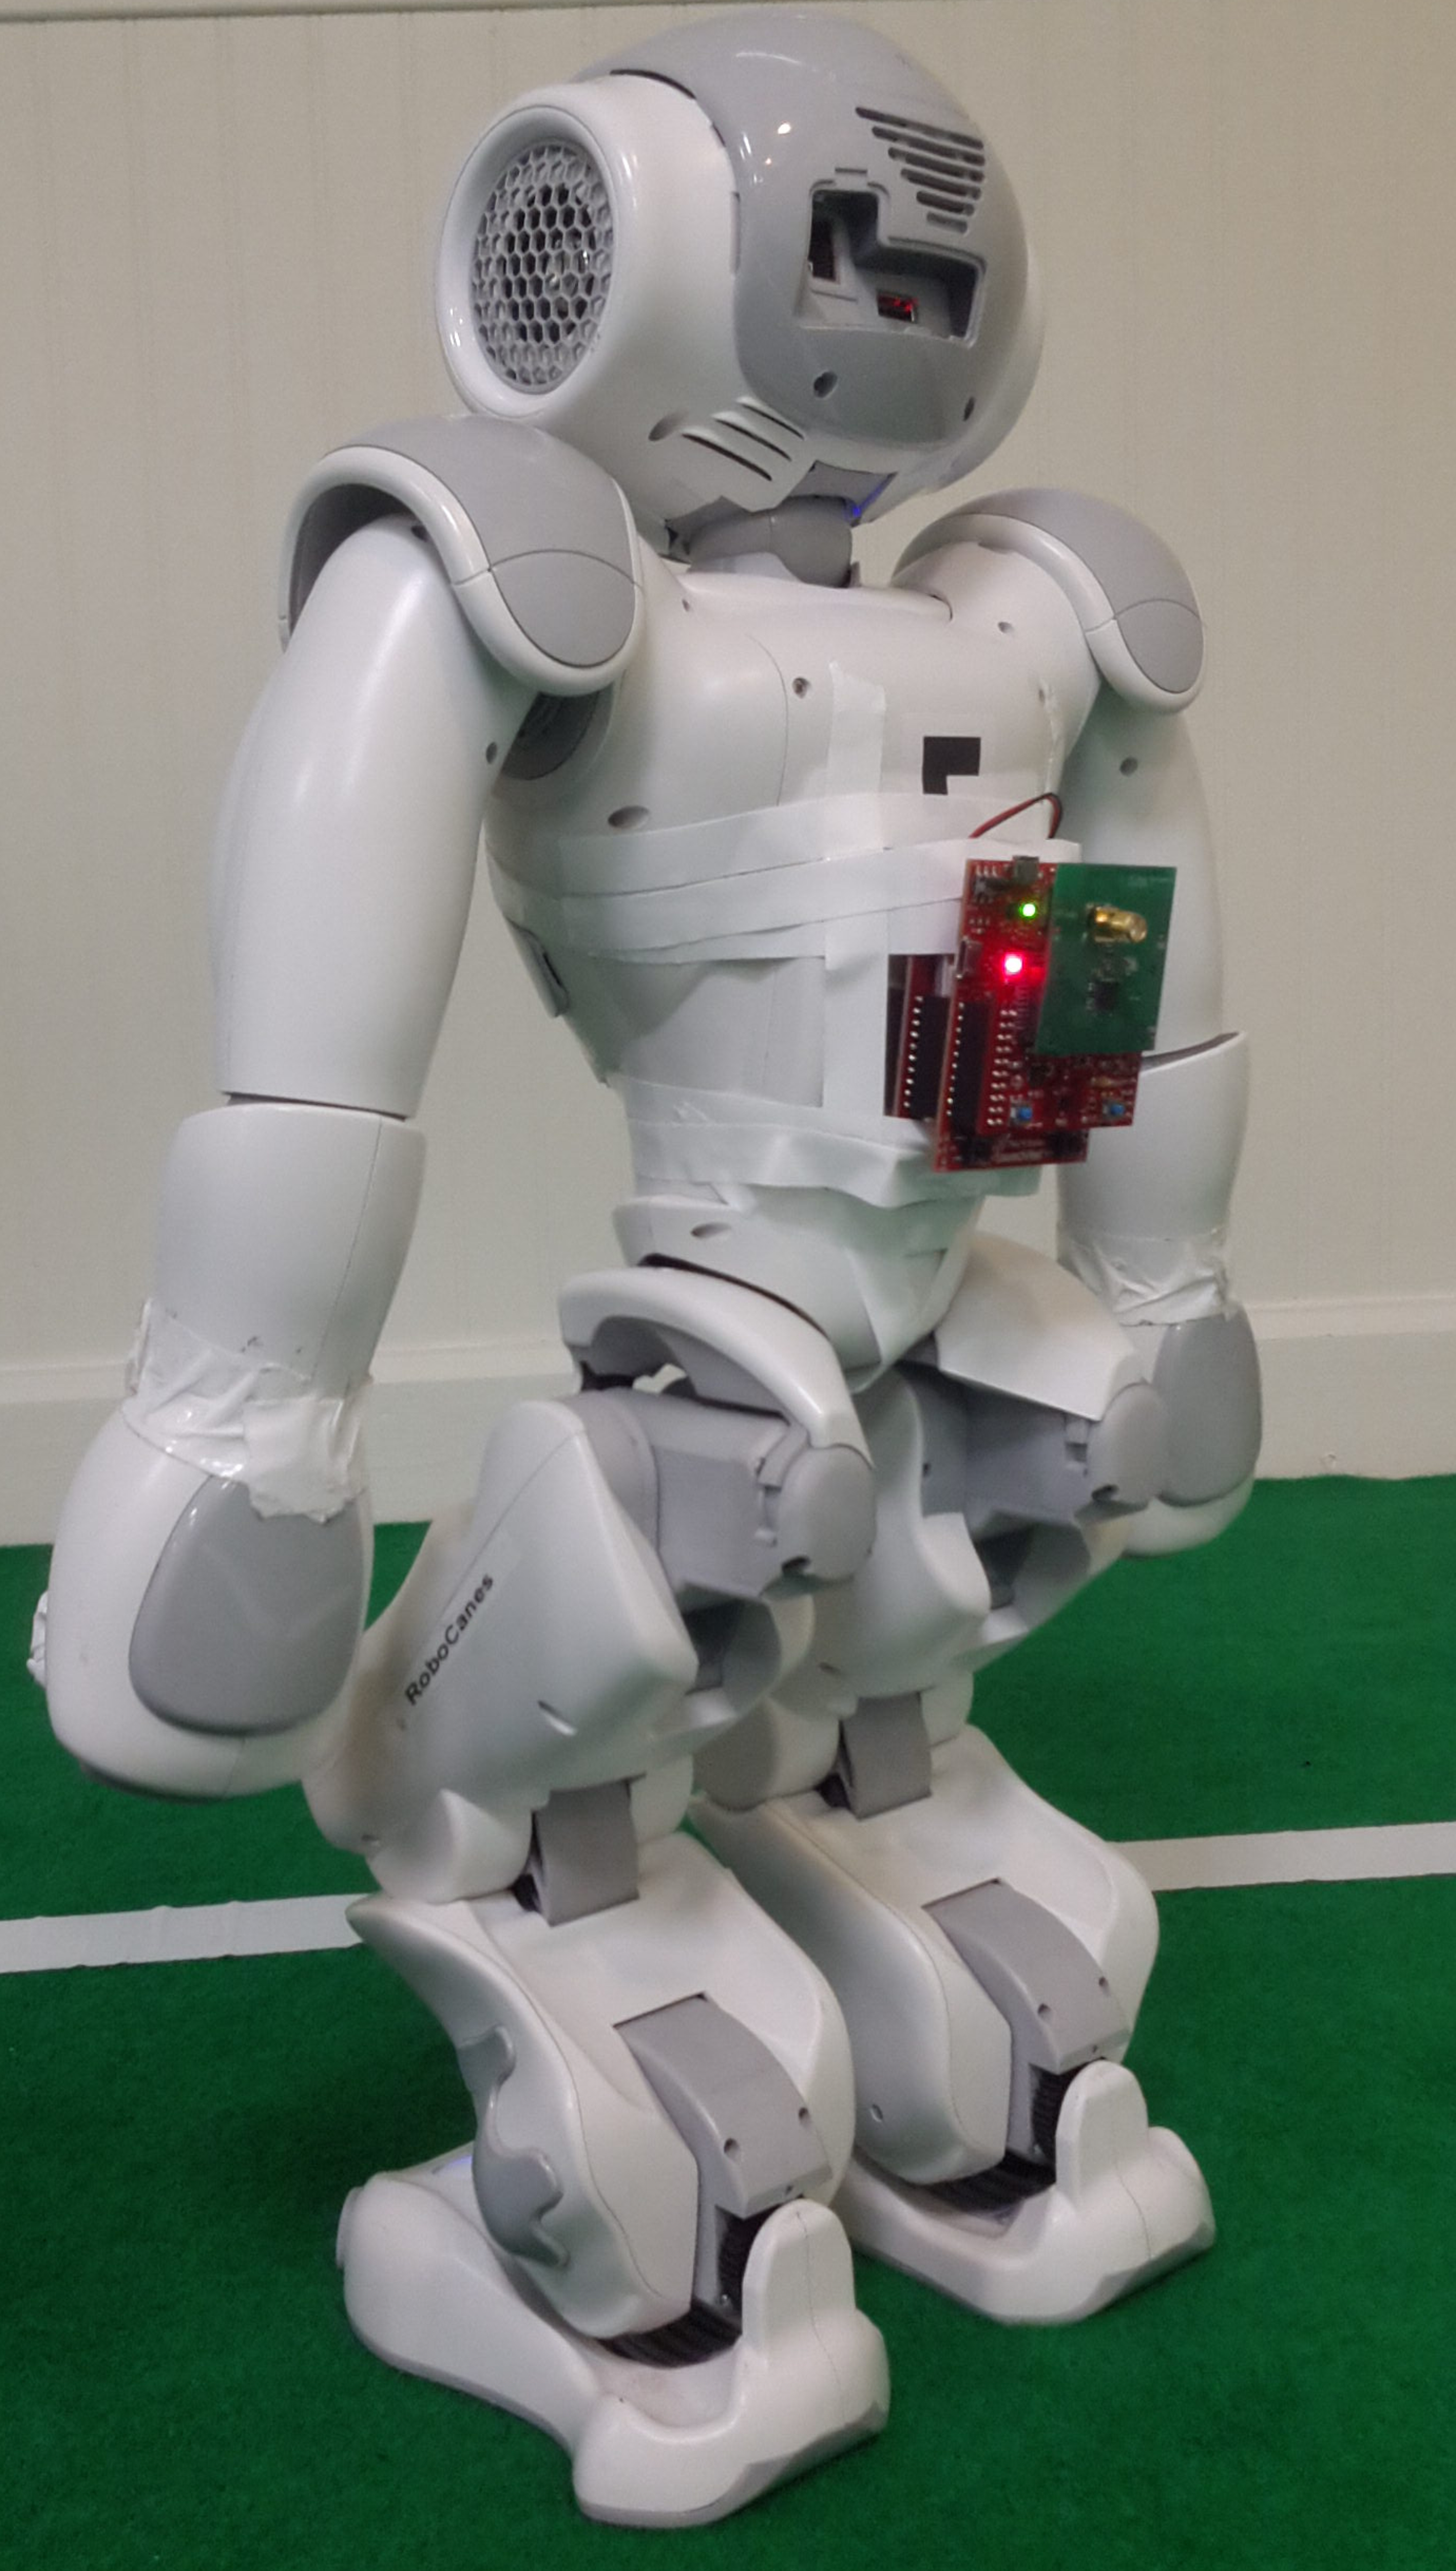
\includegraphics[width=0.4\columnwidth]{figures/robot_figure.eps}} 
\caption{(a) a wireless sensor device (assembled from a TI Tiva C Series  TM4C123G LaunchPad, a Sensor Hub BoosterPack, a CC2533 BoosterPack, and a Fuel Tank BoosterPack) attached to the back of a human subject; the device is running our framework  with only three motion-sensing modules; and (b) the 
same device configuration was used on the back of a NAO humanoid robot.}
 \label{fig:deviceWithSubjects}
\end{figure}

\subsection{Our Approach and Contributions}

Many off-the-shelf hardware boards, such as, TI microcontroller boards (MSP430{\texttrademark}LaunchPad, Tiva{\texttrademark} C Series 
TM4C123G LaunchPad, Tiva C Series TM4C129 Connected LaunchPad) and add-on  BoosterPacks   with sensors as well as  wireless transmitter and receiver  provide flexible platform for 
developing smart-devices for a wide rage of low power and portable applications. For our experiments, 
we have assembled a wireless sensing-device with a Tiva C Series TM4C123G microcontroller board, and three 
boosterpacks --- a
Sensor Hub BoosterPack  for sensing 9-axis motion,  a CC2533  BoosterPack for wireless 
networking, and a Fuel-Tank BoosterPack for power. We also assembled a wireless data collection device with a Tiva C Series TM4C123G microcontroller board, and a  CC2533  BoosterPack. These two devices were networked to create a wireless sensor network (WSN) for 
collecting motion data from  humans and NAO humanoid robots. The data collection device is connected to a computer with a USB cable for logging sensed data.   

We have developed a set of software tools to create a framework that allow us
\begin{inparaenum}[($i$)] \item  to setup the WSN, \item to collect data, \item to extract training examples from sensor readings, \item to learn from sample examples, and \item 
to monitor and predict events. \end{inparaenum} This framework is general enough for other practitioners to use the
available functionalities for creating WSNs, collecting data, learning, and prediction.

The rest of the paper is organized as follows. In Section~\ref{sec:framework}, we describe the software development 
framework that we have proposed and implemented.
Section~\ref{sec:SemiAutomaticExtractionOfTrainingVectors} reports our novel methods for  
semi-automatic extraction  of \begin{inparaenum} [($i$)] \item training samples to be 
used by the learning algorithms  and \item testing data for activity monitoring. 
\end{inparaenum} Outlines of offline leaning algorithms used for teaching the device to 
identify activities and fall events are described in Section~\ref{sec:OffLineLearning}. 
 In the penultimate section, we present detailed description of evaluation of proposed methods and also, report some typical results for humans and NAO humanoid 
robots. 
%We have utilized two machine learning algorithms and a thresholding based method to learn 
%and identify normal and abnormal activities. Then we also have presented our observations and 
%discussion. 
Finally, the paper is concluded with a summary and future work.  

\section{Related Work}
\label{subSec:relatedWork}

The modern activity detection methods can be broadly categorized in to two groups based on: 
\begin{inparaenum}[($i$)] \item inexpensive wearable embedded devices; and \item smart-phones. 
\end{inparaenum} Wearable embedded devices with add-on sensors provide options to develop effective 
activity recognition methods for humans and biped humanoid robots alike. The existing activity 
detection methods focus on special cases of fall detection in humans and humanoid robots. These 
methods were primarily used in isolation.  Using readings from accelerometer and gyroscope a methods for detecting four fall events --- forward, backward, right, and left - was reported in \cite{ojetolaFallDetection2011}.  Reported method utilized  a decision tree to 
learn and classify falls and activities of daily living (ADL). The method identified fall events 
with precision of 81\%  and recall of 92\%. 

Detection method reported in\cite{baekFallDetection2013}, used necklace-shaped tri-axial
accelerometer  and  gyroscope  sensors  for classifying  the  behavior  and  posture  of  human
 subjects. Their method distinguished between  ADLs and  falls, with  sensitivities  greater  than 
 80\%  and specificities  of  100\%. They experimented with ADLs such as: standing, sitting in the 
 chair or floor, laying, walking, running, going upstairs/downstairs, and bending, while, 
 falling forward, backward, leftward, rightward, and fall on the stairs were treated as abnormal 
 events. 
 
\cite{leoneFallDetection2013} prosed a system to detect event that cause trauma, and disabilities
using a tri-axial MEMS wearable wireless accelerometer. They used support vector machine (SVM) for
robust classification of different events. \cite{BaoActivityrecognition2004} reported of using five 
small biaxial wire-free accelerometers attached  on the left bicep, right wrist, left quadriceps, 
right ankle, and right hip to recognize 20 activities starting from  walking  to  riding elevator  
to  strength  training to bicycling. They reported using decision table, instance-based learning, 
decision tree, and na\"{i}ve Bayes classifiers, where, decision tree showed the best performance 
with 84\% accuracy.  Similar efforts have been reported to detect human motions using motion 
tracking, e.g., 
\cite{dumitracheFallDetection2013,kumarActivitAndFallDetection2013,krishnanActivityRecognition2014,gaoActivityRecognition2014,alvarezActivityAndFallRecognotion2015}.
 


{~\cite{moyaFallAndDamageDetection2015}} proposed a fall detection, avoidance, and damage 
reduction mechanism for biped humanoid robots. They tried to simulate the real world environment 
where humanoid robots have to walk over irregular surface, running or playing sports, collision 
with other robots. Their framework detected instability and performed fall avoidance or at 
least low-damage falling mechanism was invoked. Therefore, embedded devices  with add-on sensors 
provide a flexible platform to build may real world applications. 


There is an increasing popularity in using smart-phones to detect activities in health care domain. 
Using only the accelerometer readings from a smart-phone, \cite{baiFallDetectionPhone2013} analyzed five 
actions of human walking, running, standing up, sitting down, and jumping. They compared the 
acceleration characteristics of these actions with three different fall accelerations to infer the 
direction of the fall. Their method recognize the fall activity, only when a predefined set of 
conditions were met. But the method did not provide any prediction or indication value, that a fall 
may occur in future. 

\cite{steidlFallDetection2012} reported that the sensors of the smart-phones from different manufactures 
record values significantly incompatible ranges for identical tasks. Therefore, they trained a SVM 
classifier based on the features extracted from raw accelerometer readings and the directional 
changes of the constraining force exerted on an accelerometer to detect fall events. They compared 
these events to non-fall activities such as walking, running, jumping, and some actives which 
resembles falls such as sitting down on a chair. Their method detected fall events 84.8\% average 
accuracy across different smart-phones. 

\cite{DernbachActivityAndFallDetectionPhone2012} explored methods to detect simple and complex activities using inertial 
sensors (accelerometer and gyroscope) of an Android smart-phone. The simple activities included: 
biking, climbing stairs, driving, running, sitting, standing, walking, and state of the phone not 
on the person. The complex activities were: cleaning, cooking, medication, sweeping, washing hands, 
and watering plants. Six different classifiers, multi-layer  perceptron (MLP), na\"{i}ve  Bayes,  
Bayesian  network,  decision  table,  best-first tree, and  K-star,  were trained on using the same 
feature extractor. For simple activities, 93\% accuracy using MLP were reported, while, 50\% 
success was achieved for complex activities.    

\cite{ShenFallDetectionPhone2015} used a  high-level fuzzy Petri net for the analysis and the development of 
identifying normal human actions such as sitting-down, squatting, walking, running, and jumping and 
abnormal events such as falling forward, backward, sideways, and vertical. Their fall detection 
method reported 94\% accuracy. One disadvantage of their process was that, some complex situations 
and movements cannot be detected accurately; e.g., falling down from  stairs, multiple collisions, 
or temporal unbalance motions.

\par 
To the 
best of our knowledge only a three studies have been dedicated to biped robots \cite{Andre2015,Goswami2014,Moya2015}. The focus for these studies were prediction of a fall before it occurs and taking corrective measures to prevent the fall. The work reported in these papers are using readings from multiple sensors embedded in a robot for predicting potential fall. On the other hand, our research goal is identification of fall and non-fall events after it occurs.


%Similar to existing methods, we have defined different normal and abnormal activities for humans 
%and NAO humanoid robots. In order to validate our hypotheses that the learning and predicting 
%methods unifies across the two groups, firstly, we have restricted the activities that can be 
%performed on a NAO robot. Therefore, in our experiments, the human performed activities that are 
%similar to the robot, such as, walk or falling forward/backward so forth. Secondly, we have 
%extended the human activities to more complex events.  We have used Texas Instruments 
%(TIs)  microcontrollers and boosterpacks for our experiments, 
%but, one can use microcontrollers and  sensor boards from other sources.  




\section{Framework for Data Collection and Processing}
\label{sec:framework}

A real-time or near real-time monitoring device performs a sequence of $n$ tasks $T = \{ T_1, T_2,\cdots,T_n\}$. A task $T_i$ may depend on another task $T_j$.  For satisfying dependence of a task on other tasks, it is necessary to create an \emph{execution order} on the set of tasks, if one exists. Denoting dependence of $T_i$ on $T_j$ as $D_{ij}$, a directed graph $G(T,D)$ can conveniently describe dependance among the tasks. A list of dependencies $D_{ij}$ completely describes the graph $G(T,D)$.
\par
We have created a generic framework for developing applications for \emph{data collection and processing}. This framework is described next.
%TODO: write an introduction paragraph for the section. For convince of reference for 
%Framework for Data Collection and Processing will be denoted by  FDCP. 

\begin{figure*}[!t]
\centering
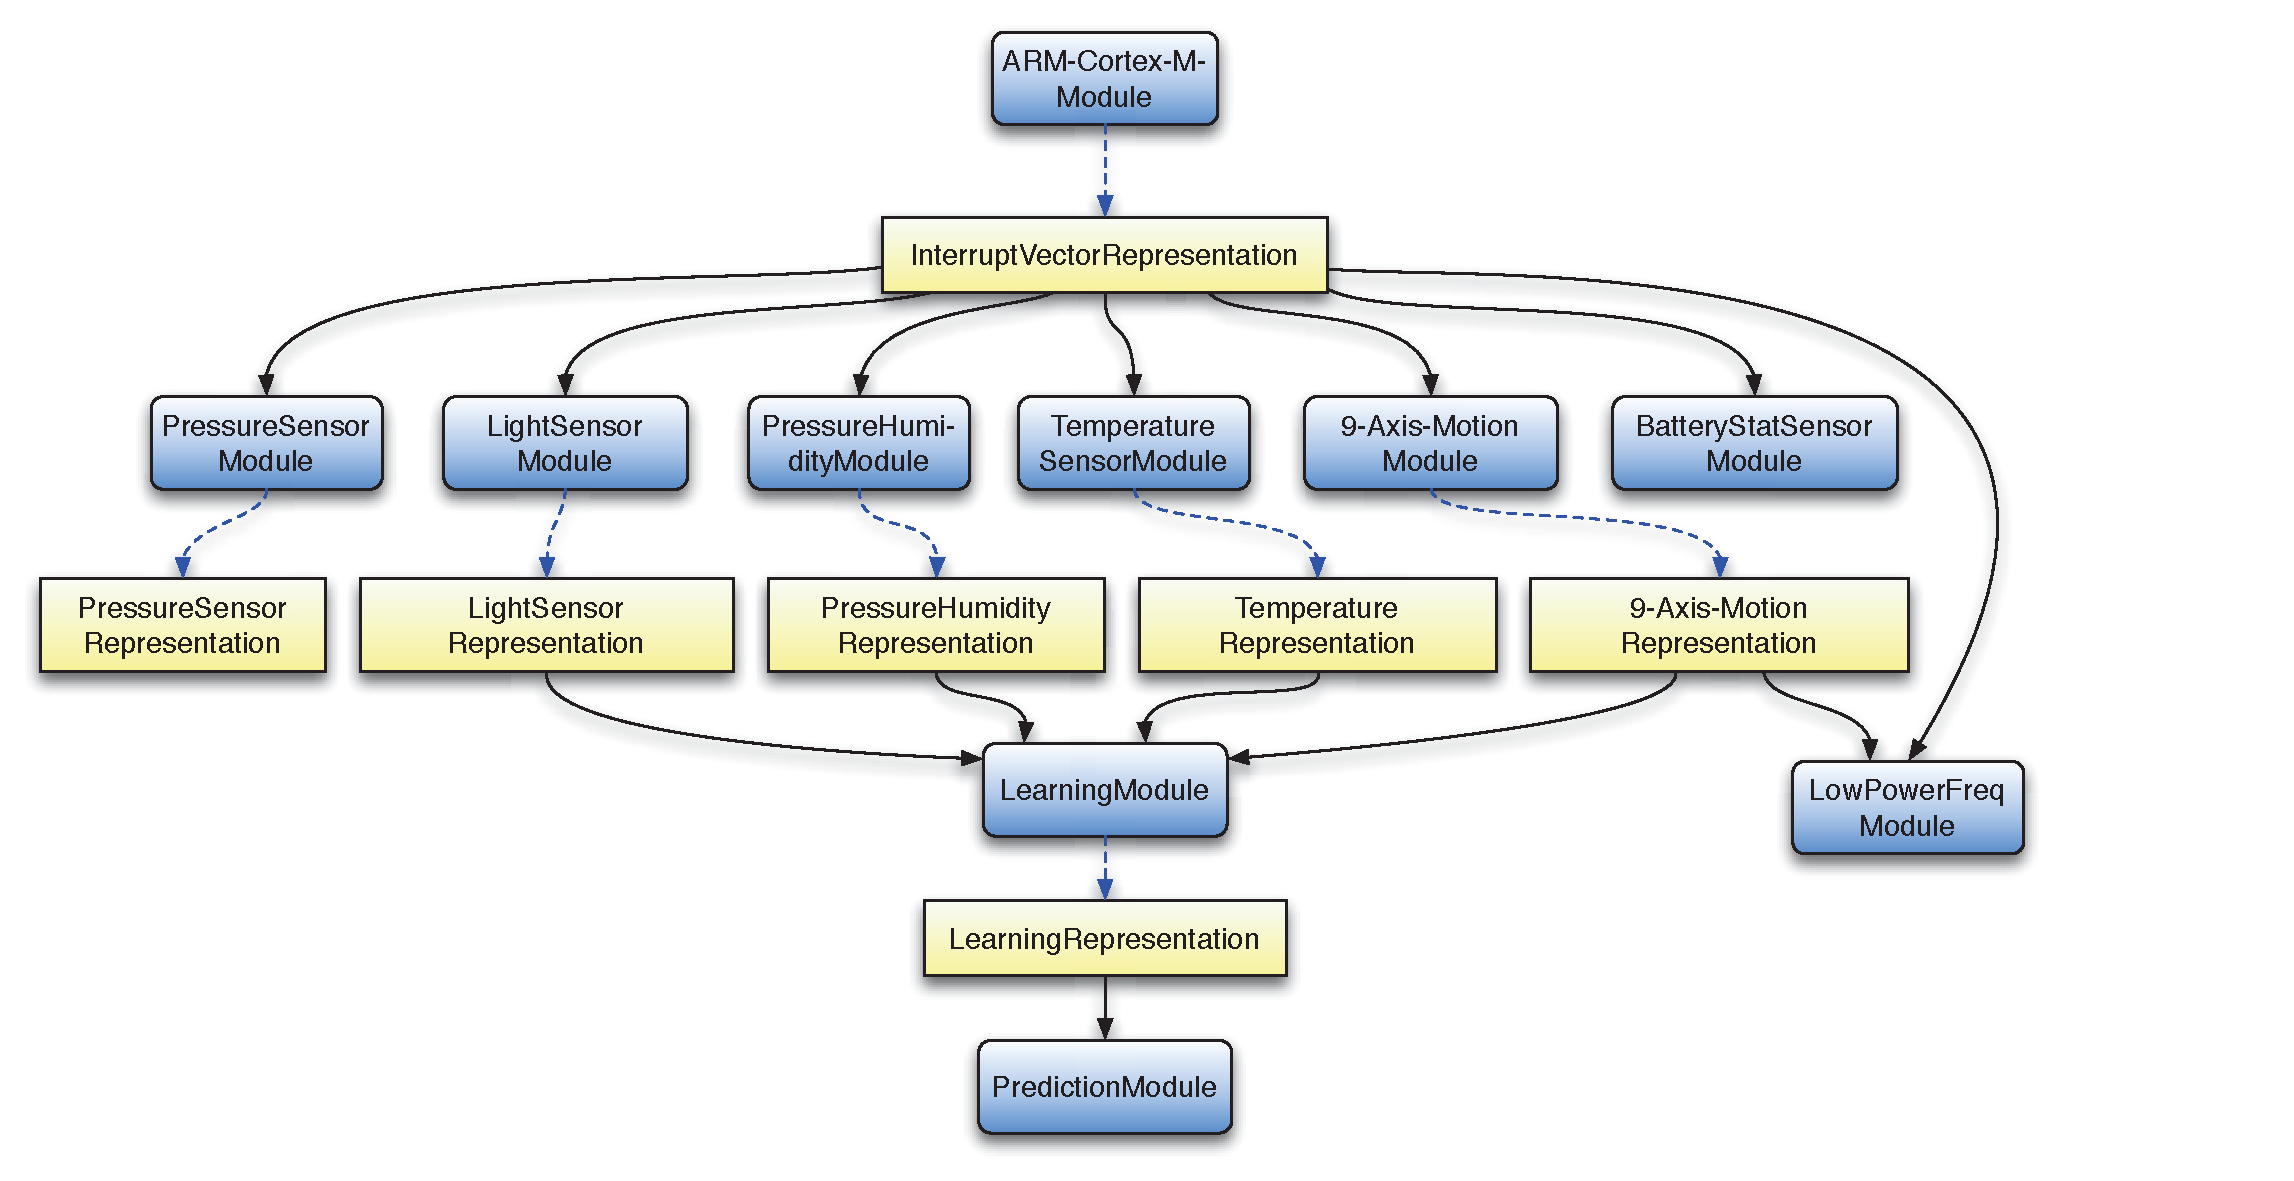
\includegraphics[width=\textwidth]{figures/graph_structure_def-crop3.eps}
\caption{Currently available software modules in our framework and a directed-graph representation of their functional relationship. Execution of a module (rounded-corner rectangle) generated data that is stored in the representation module (pointed-corner rectangle) for feeding into the next module.}
 \label{fig:framework}
\end{figure*}

\subsection{Overview of the Framework}
\label{sec:OverviewOfTheFramework}

\par
The framework provides generic functionalities to develop applications or rational agents 
on embedded devices that sense and actuate using add-on boards. The execution paths between sensors 
to actuators could contain complex behavior manipulations and modeling decisions that needs to be 
developed efficiently.
The framework 
includes: \begin{inparaenum}[($i$)] \item tools to develop modules and representations that execute on 
the microcontrollers or offline, \item the methods to access functionalities for physical 
robots, 
and \item a real-time visualization system\end{inparaenum}. Our framework is lightweight, flexible, 
and consumes minimum memory and computational resources. We have tested our framework on multiple 
microcontrollers and on boosterpacks. 
Our development framework, $\mu$Energia (\textit{pronounced as}: ``micro--Energia'') is availabe from
\textit{site}:
{http://muenergia.saminda.org}.

\subsection{Task-Schedule Generation Using our Framework}
\label{FrameWorkDescription}

%TODO: write what is meant by ``ordering''

 For ease of description and clarity of understanding, we have divided each task into two components: a {\em module} and one or more {\em representations}. A module implements executable code, while a representation exchange information from one module to another. Thus, a module may generate information for multiple representations as well as it may get inputs from multiple representations. 
\par
Once a user provides dependency descriptions, the framework converts it  into a directed graph (also know as precedence graph, or conflict graph).  If the graph has no cycle, the framework topologically sorts the nodes and creates an schedule for execution of the modules. In case there the graph has one or more cycle, the framework reports so to the users.
For visualization of schedule, the framework  generates a directed graph. In this graph, modules are drawn as blue-shaded rectangles with rounded corners and the representations are drawn as yellow-shaded rectangles with pointed corners. The dependence of a modules on a representation is depicted as with a black arc with a solid line, while the dependency of a representation on a module is depicted with a blue arc with a dotted line. We have tested our framework on multiple 
microcontrollers and on boosterpacks.

Directed graph in Figure \ref{fig:framework} shows a framework generated task-schedule for  a TI Tiva C Series TM4C123G microcontroller to collect and process data from \begin{inparaenum}[($i$)] \item Bosch Sensortec BMP180 pressure sensor, \item Intersil ISL29023 ambient and infrared light sensor, \item Sensirion SHT21 humidity and ambient temperature sensor,  \item  TIs TMP006 non-contact infrared temperature sensor, and \item InvenSense 
MPU-9150 --- a 9-axis MEMS motion sensorthee-axis. \end{inparaenum}

%\par
%The framework 
%includes: \begin{inparaenum}[($i$)] \item tools to develop modules and representations that execute on 
%the microcontrollers or off-line, \item the methods to access functionalities for physical robots, 
%and \item a real-time visualization system\end{inparaenum}. Our framework is lightweight, flexible, 
%and consumes minimum memory and computational resources. We have tested our framework on multiple 
%microcontrollers and on boosterpacks. 
%Our development framework, $\mu$Energia (\textit{pronounced as}: ``micro--Energia'') is availabe from
%\textit{site}:
%{http://muenergia.saminda.org}.


\subsection{An Application of the Framework}

%The Figure \ref{fig:fa} shows the modules and representations related to our 
%experiments, where the boxes represent the computational modules, while the rounded-boxes represent 
%the input to a module or an output from a module. For brevity, in the rest of the paper, the  
%{\em computational modules} are refereed as  {\em modules}. 
Our current project use 
the module {\em 
9-Axis-Motion Module} that contains logic to read from or write to MPU-9150, a 9-Axis 
(Gyro+Accelerometer+Compass) MEMS MotionTracking device on the sensor hub booster pack. The {\em 
9-Axis-Motion Module} deposits data from the motion sensors to 
representation {\em 9-Axis-Motion Representation}, which are used by the {\em 
Learning Module}. The {\em LeaningModule} use the motion sensor data and creates {\em LearningRepresentation} for the {\em PredictionModule}. 

\par 

In the next section we propose a method for semi-automatic extraction of training examples from motion datasets. These examples are used to teach a device/system that identifies desired events. 

\section{Semi-Automatic Extraction of  Training Examples}
\label{sec:SemiAutomaticExtractionOfTrainingVectors}

This section provides our main contribution of the paper. We provide a detail description 
of the semi-automatic training examples extraction method, which has expedited the 
annotation 
of motion data considerably. In our study, we have considered four types of fall events: 
\begin{inparaenum}[1)] \item fall forward ({\sf FF}), \item fall backward ({\sf FB}), 
\item fall left ({\sf FL}), and fall right ({\sf FR}). \end{inparaenum} We have used the 
following seven activities:\begin{inparaenum}[1)] \item walk forward ({\sf WF}), \item 
walk backward ({\sf WB}), \item walk left ({\sf WL}), \item walk right ({\sf WR}), \item 
marching ({\sf MR}), \item rotate counter clockwise ({\sf RC}), and \item rotate 
clockwise ({\sf RA})  \end{inparaenum} as non-fall activities. 


 
%TODO: we need an introductory paragraph describing a set of activities $A = \{A_1, A_2, 
%\dots, A_n\}$. Show unfiltered data sample for couple for fall and non-fall time series. 


\subsection{Preprocessing of Data Collected with Motion Sensors }
\label{subsec:preDataCollection}

We have setup the framework as described in Section \ref{sec:framework} and enabled the 
motion tracking device to sample at $20$ ms, which is equivalent to 50$Hz$ 
sampling rate. The motion tracking device outputs nine values. The  
accelerometer readings are in  meter per square second ($m/s^2$), gyroscope readings are 
in 3-axis in radian per square second ($rads/s^2$), and the magnetometer readings are  in 
Tesla ($T$). For our experiments, we have excluded the magnetometer readings. Therefore, 
our input vectors are in $\mathbb{R}^6$, which consist of accelerometer and gyroscope 
values.

\begin{figure}[htb]
	\centering
		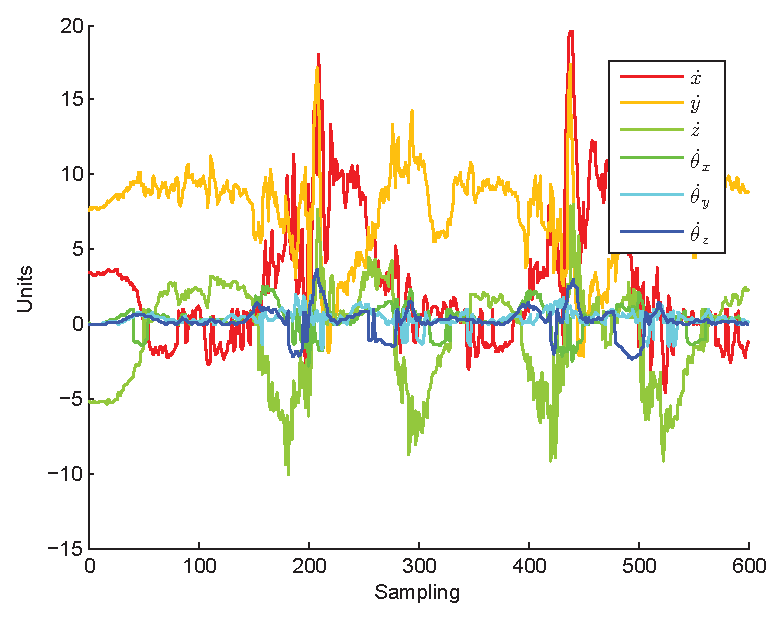
\includegraphics[width=0.95\columnwidth]{plots/human_falling-crop.eps}
	\caption{Motion dataset for  Fall Forward event of a human subject}
	\label{fig:human_falling-crop}
\end{figure}


\subsubsection{Identify and Adjust for Missing Data Points}
\label{sec:IdentifyAndAdjustForMissingDataPoints}
Some data packets may be lost during transmission because of noise. We numbered each 
sensor reading sequentially and lost data points were identified from this number and was 
replaced using linear interpolation. Since only very few data points were lost and 
results obtained after linear interpolation was excellent, we did not experiment other 
interpolation method.

\begin{figure}[htb]
	\centering
		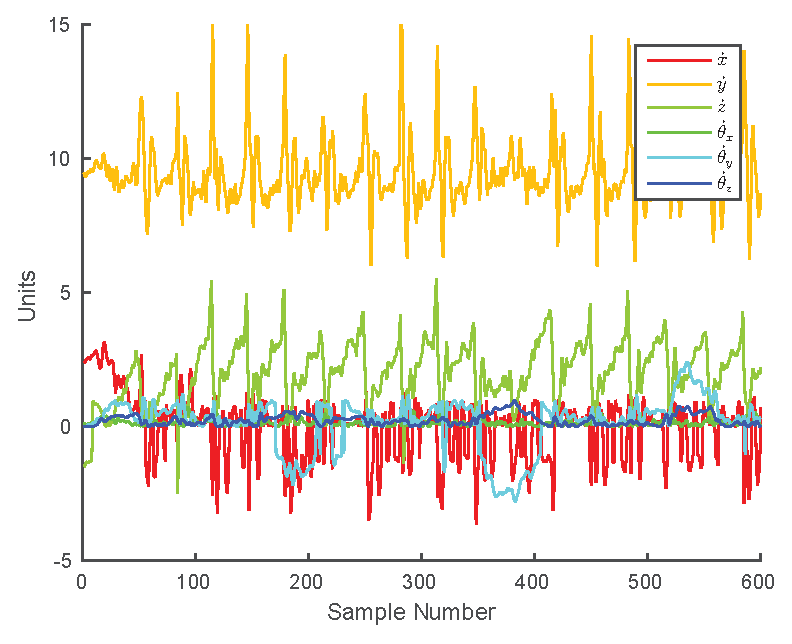
\includegraphics[width=0.95\columnwidth]{plots/human_walk-crop.eps}
	\caption{Motion dataset for Walk Forward event of a human subject. }
	\label{fig:robot_fallen_forward-crop}
\end{figure}


\subsubsection{Noise Filtering}
\label{sec:NoiseFiltering}

After checking for missing data and adding interpolated values for lost data,  high frequency noise was removed using a moving window averaging technique. We used a window  of 20 consecutive samples, which amounts to 400$ms$, 
and obtain the average value. Then the  window was moved by 10 samples, then average was and 
repeated the process. Therefore, we have allowed 10 samples to overlap between windows. 
Selection of 10 samples overlaps is based on our empirical observation that a transition from non-fall event to a fall event is about 500$ms$. Thus, averaged values will preserve transitions from non-fall events to fall events.   We have used the preprocessed stream as the input to our automatic training example 
extraction method.


\subsection{Semi-Automatic  Extraction Training Examples}

Barrier for collecting motion data is very low, if any. But, detection and identification of activities and fall events from motion data has remained an active area of research, as can be seen from recent list of publications. The main unsettled issue is how to characterize features from motion data that can be extracted easily for training and monitoring. In this section, we describe a method that semi-automatically extracts feature vectors that characterize activities and fall events.

The flow chart of method used for extracting training examples are shown in Fig.~\ref{fig:FlowChartforAlgorTrainingExamples}. All the collected data sets were annotated. If a dataset was for simulated fall events, the dataset was treated as a 6-dimension vector for clustering them into two clusters. We used K-Mean and Gaussian Mixture clustering techniques. For completeness a brief description of each is provided next.

%TODO: first paragraph => why we need SATEE. Because of the difficulty of generating 
%training data. Then, description of the algorithm, with the figure (training data only). 
\begin{figure}[htb]
	\centering
		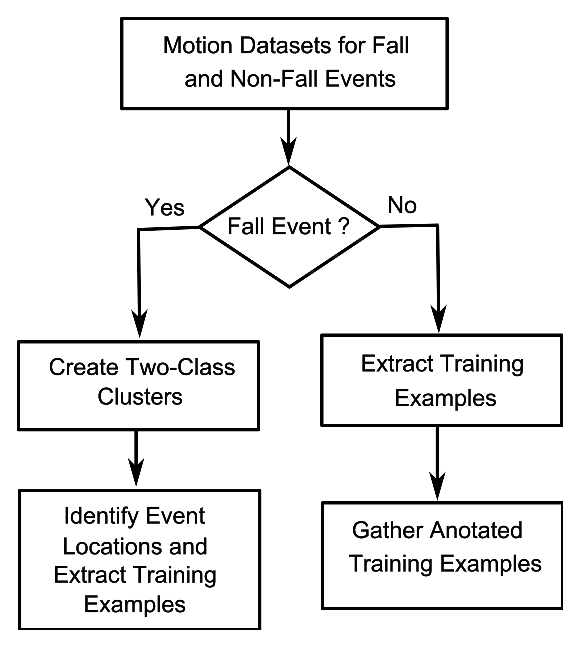
\includegraphics[width = 
		0.84\columnwidth]{figures/FlowChartAlgoForTrainingExamples.eps}
	\caption{Flow chart of an algorithm for semi-automatic extraction of training examples}
	\label{fig:FlowChartforAlgorTrainingExamples}
\end{figure}

\subsubsection{K-Mean Clustering}
K-mean clustering aims to partition a set of $n$ observations into $k$ clusters. Each 
observation is assigned to the cluster with the nearest mean. Let 
\{($\mathbf{x}^{(i)}$)\}$_{i=1}^n$  be the set of $n$ 
observations, where each observation $\mathbf{x}^{(i)}$ is a $d$-dimensional real vector 
and is 
assigned to one of $k$ sets $\mathrm{S}_j \in \mathcal{S}$, for $ 1 \leq  j \leq k$ so 
that 
within-cluster 
sum of squares is minimized. Formally,

$$ \min _{\mathcal{S}} \sum_{i=1}^{k} \sum_{\mathbf{x} \in \mathrm{S}_i} || \mathbf{x} - 
\boldsymbol{\mu}_i 
||^2,$$
where $\boldsymbol{\mu}_i $ is the mean of points in $\mathrm{S}_i$.

For our case, we set $k = 2$ for extracting  training examples for fall events. The 
clustered samples are shown in Figures~\ref{fig:automatic_annotation} and 
\ref{fig:automatic_annotation2}. For our fall event datasets, the choice of $k=2$ is the 
optimal value that clearly separated the duration of the fall. 


\subsubsection{Multivariate Gaussian Mixtures}

Gaussian mixture clustering is a generalization of k-mean clustering, where each cluster 
is assumed to be from a Gaussian distribution parametrized by $\boldsymbol{\mu}_k, 
\boldsymbol{\Sigma}_k$. The mean vector $\boldsymbol{\mu}_i$ represents the center of the 
cluster $i$. 
Usually an \emph{expectation maximixation} (EM) algorithm iteratively identifies the 
clusters. Compared to the clustering obtained from k-mean, the mixture models did not 
provide an optimal separation for our fall datasets. Therefore, we have only used the 
clustering obtained from 
k-means algorithm to extract the training examples. 
 

The activity annotation is an arduous and cumbersome process. As we have mentioned in 
Section \ref{subSec:relatedWork}, the previous methods favor manual activity annotation, 
which has been the single most time consuming part of the training example gathering 
process. We present a semi-automatic activity annotation methodology based on 
clustering, which has 
significantly alleviated the time to generate samples. 

Our method is relatively simple and easy to implement in practice. We have used the 
samples from the preprocessing stage, and subjected them to k-means algorithm 
\cite{Bishop06a}. We have empirically found that the minimum cost separation is 
achievable when we have two clusters. This intuitively supports the fall event datasets 
as well. For 
example, if we consider the falling forward event, there is a window in which the fall 
triggers and the subject falls to the ground. Therefore, the signature of this process 
differs from the states before the process starts (e.g., standing) and the states after 
(e.g., laying on the floor). Therefore, each fall dataset, there exists a duration in 
which the fall triggered and continued.


\begin{figure}[!htb]
\centering
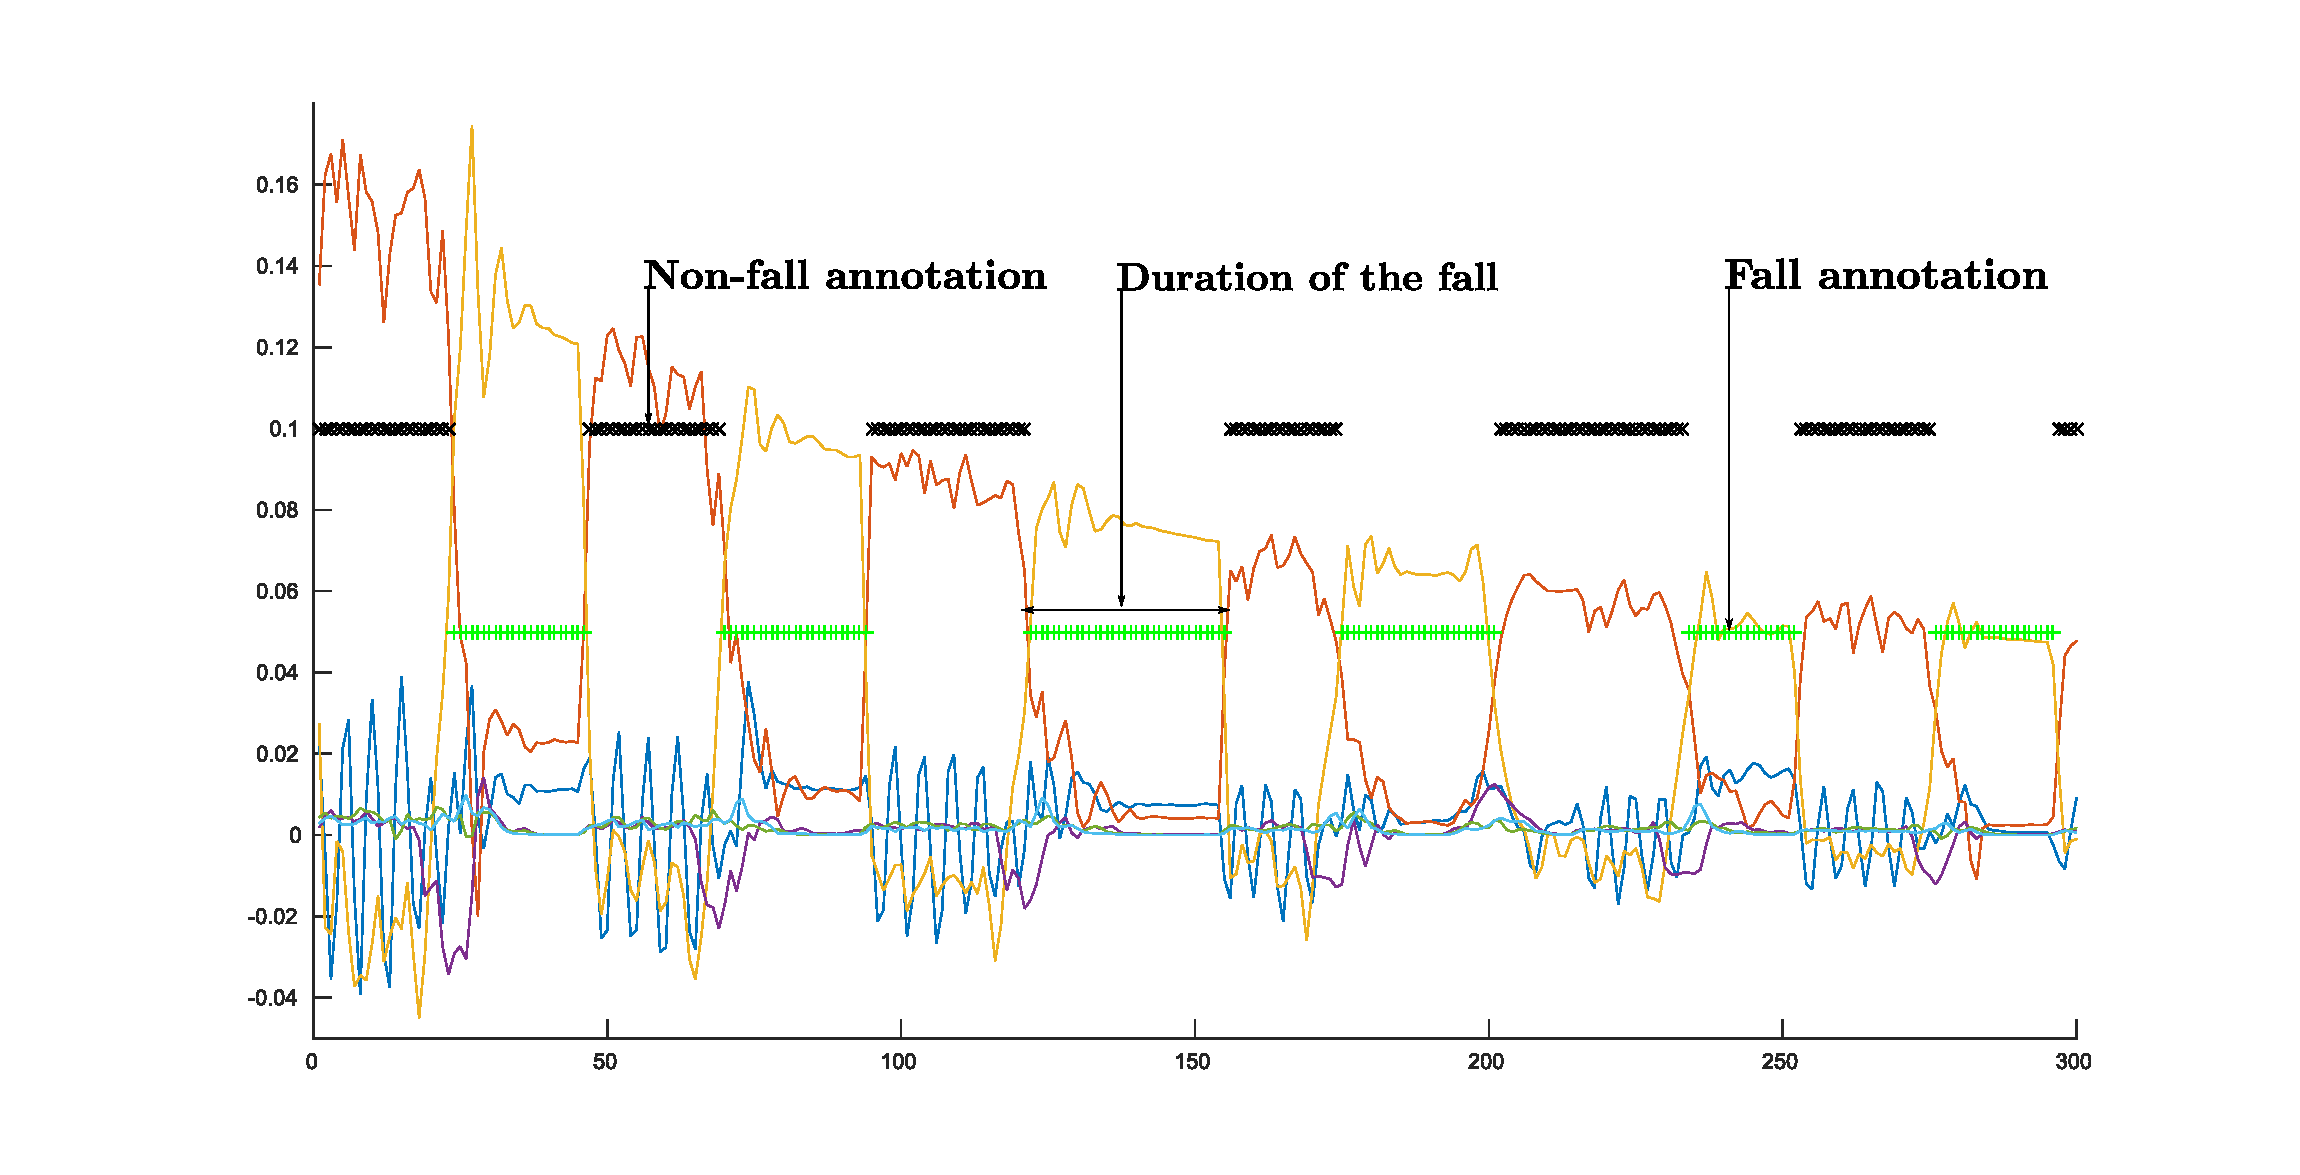
\includegraphics[width=0.48\textwidth]{plots/human_falling_forward2.eps} 
\caption{Semi-automatic annotation of falling forward event dataset.}
 \label{fig:automatic_annotation} 
\end{figure}


\begin{figure}[!htb]
\centering
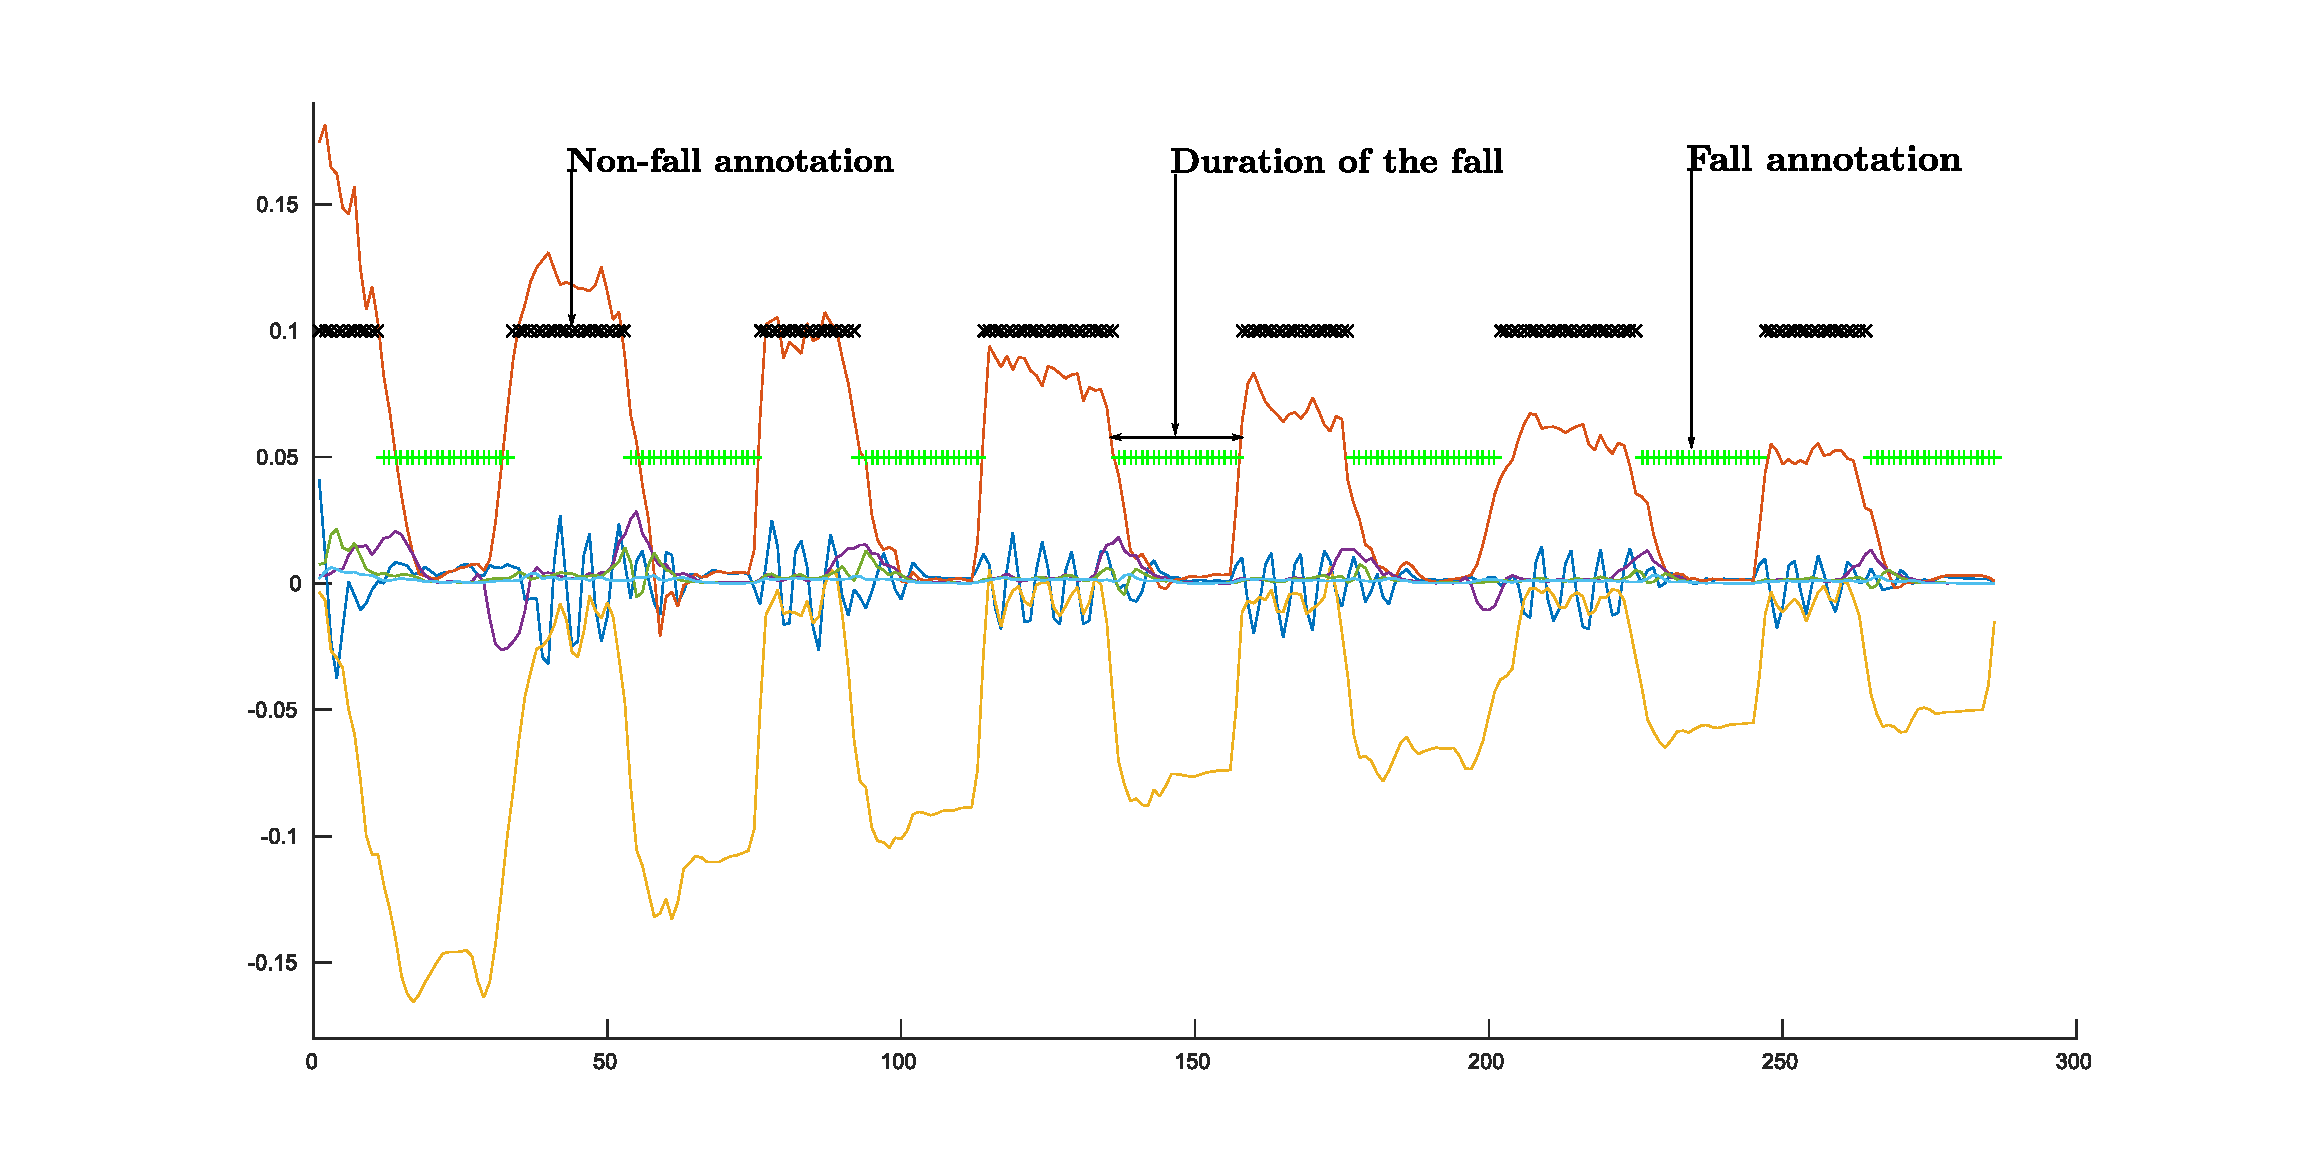
\includegraphics[width=0.48\textwidth]{plots/human_falling_backward2.eps} 
\caption{Semi-automatic annotation of falling bax event dataset.}
 \label{fig:automatic_annotation2} 
\end{figure}





%\begin{figure}[!t]
%\centering
%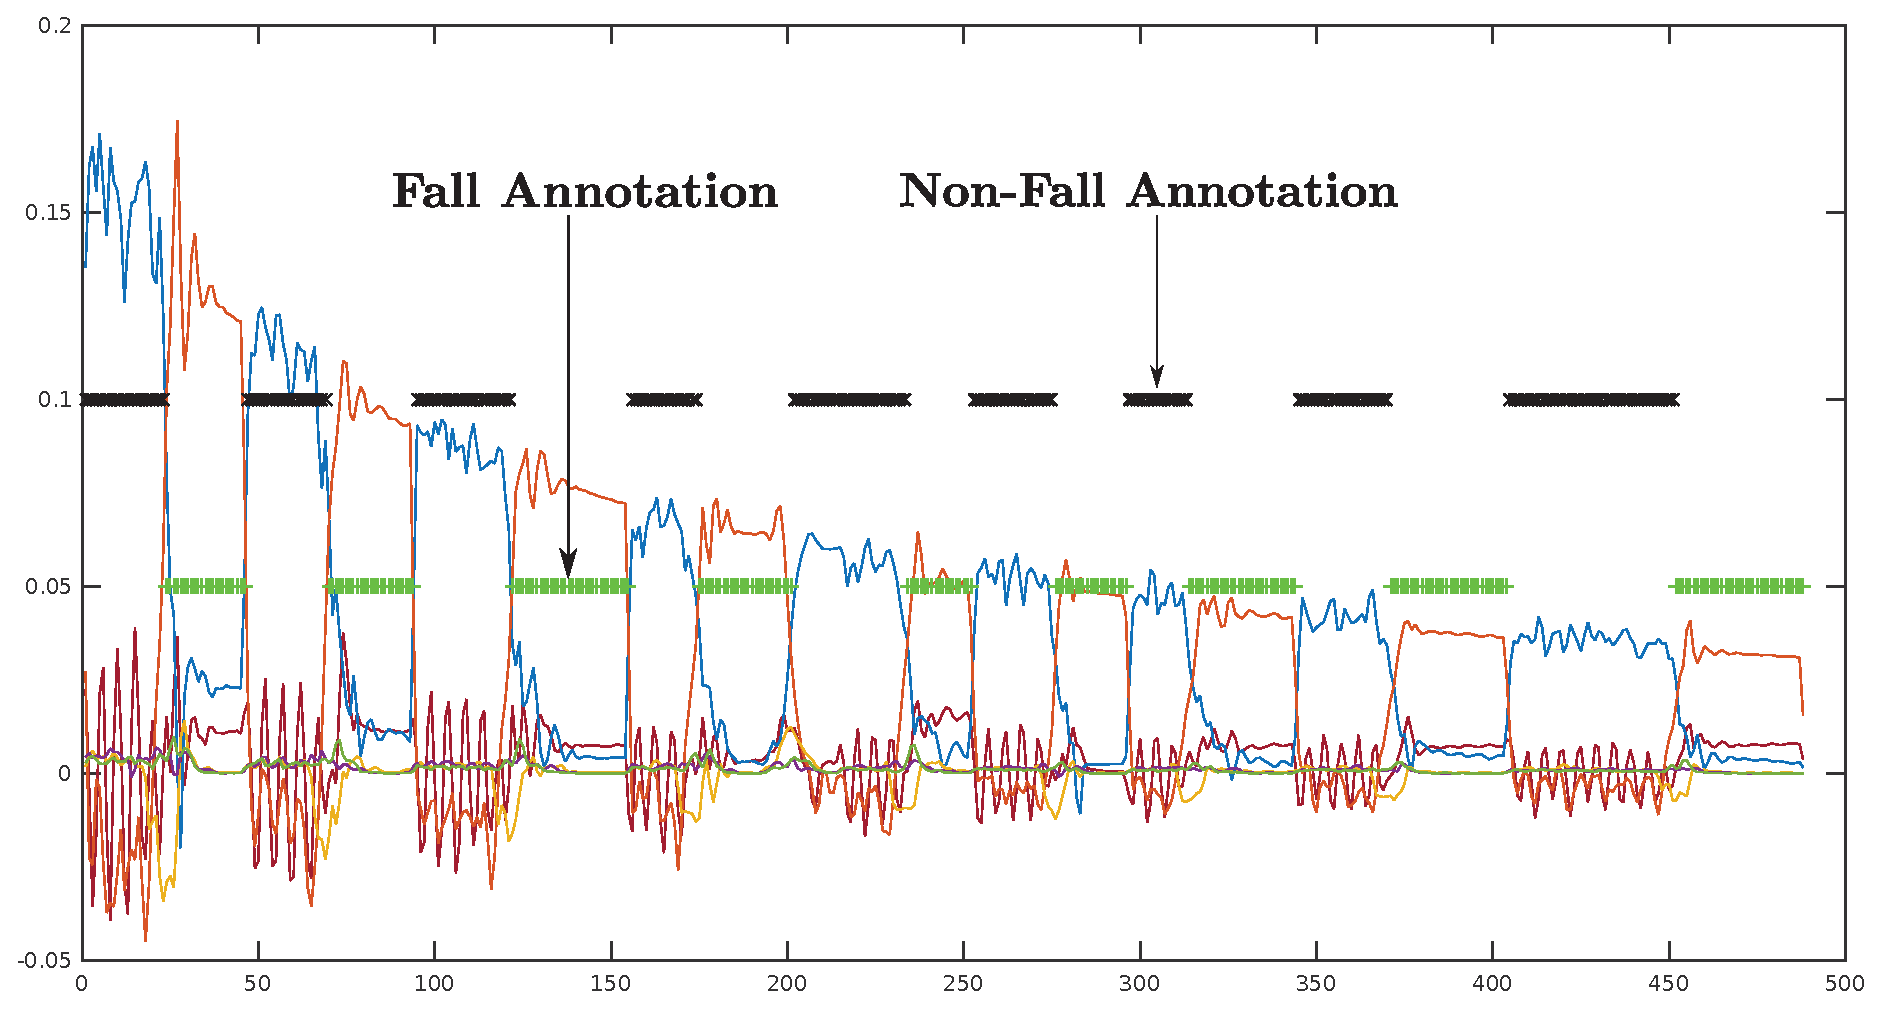
\includegraphics[width=0.48\textwidth]{figures/example_annotation-crop.eps} 
%\caption{Semi-automatic annotation of falling forward dataset.}
 %\label{fig:automatic_annotation} 
%\end{figure}


Figure \ref{fig:automatic_annotation3} shows our semi-automatic annotation of falling 
forward dataset. The subject in this experiment exercises a fall froward. After a 
fall, the subject immediately gets up and repeats the process. The green ``+'' segments 
show the annotated fall events, while the black ``x'' segments show the non-fall 
events. We have observed that there is a clear separation of the events with two 
clusters. Each segment has betweens 15 to 20 consecutive data points, which amounts to 
3000$ms$ to 4000$ms$ fall event after the triggering the event. The fall event triggers 
at the end of the non-fall segment and at the beginning of the fall segment.

\begin{figure}[!htb]
\centering
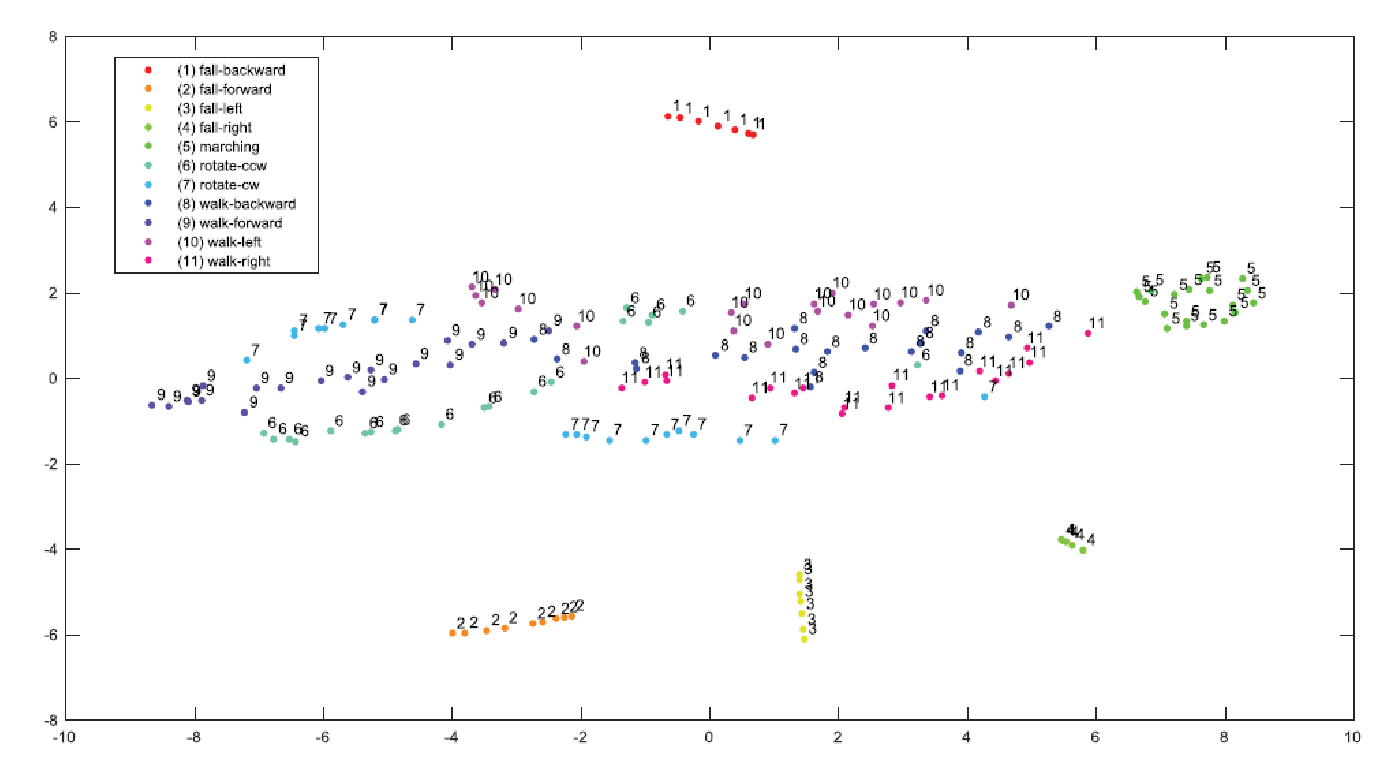
\includegraphics[width=0.48\textwidth]{figures/viz_all_training_examples_corp.eps} 
\caption{Visualization of 11 sets of training examples using Tsne projection. In this projection, the 4 fall events (numbered 1 through 4) show a clear separation from each other and other 7 non-fall events.}
 \label{fig:automatic_annotation3} 
\end{figure}


Since we are 
interested in the signature of the fall event, we have annotated all the samples belongs 
to ``a'' cluster as the fall data. The k-means clustering finds a 
local minimum in general. The cluster assignments may also vary depending on the 
initialization. Therefore, when we have obtained the data belongs to two clusters, we 
only have to manually provide the semantics of the cluster centroid. 

\section{Offline Learning and Predicting Algorithms}
\label{sec:OffLineLearning}

%TODO: About the algorithms we have used (SoftMax, ANN, and SVM).
%Trained the models using offline models. This is offline learning figure. 

Our activity monitoring and identification requires to learn and to predict beliefs of 
multiple 
discrete hypothesis. This includes learning and predicting dichotomies such as falling 
forward and 
backward, falling events and non-falling events, different types of falling events, and 
so forth. 
Therefore, 
we have used multi-class classification networks to rationally answer the question we 
have posed.

Using our semi-automated training example extraction method (Section 
\ref{sec:SemiAutomaticExtractionOfTrainingVectors}), we have created $m \in 
\mathbb{N}$ 
training examples 
\{($\mathbf{x}^{(i)}, \mathbf{y}^{(i)}$)\}$_{i=1}^m$ such that $\mathbf{x} \in 
\mathbb{R}^{n}$ 
and 
$\mathbf{y} \in 
\{0,1\}^k$. $k \in 
\mathbb{N}$ is the number of dichotomies. Each training example belongs only to one class 
and $\mathbf{y}$ uses the 1--of--$k$ coding scheme.    

\subsection{Softmax Regression Algorthm}
\label{sec:SoftmaxRegrationAlgorthm}

The first classification network is based on Softmax regression \cite{Bishop06a}. In this 
model, given an 
example $\mathbf{x}$, it will determine the probability, $\mathbb{P}(y | \mathbf{x})$, 
for 
each dichotomy $y=0,\ldots,k-1$. The input is appended with constant bias 
term, $x_0 = 1$, therefore, $\mathbf{x} \in \mathbb{R}^7$. The model uses a parameter 
matrix 
$\mathbf{W} 
\in \mathbb{R}^{7 \times k}$, and the output vector, $\mathbf{a} = \mathbf{Wx}$, is 
passed 
through 
the 
Softmax 
activation function $\mathbf{z(a)} = \frac{e^{\mathbf{a}}}{\mathbf{1}^\mathtt{T}
e^{\mathbf{a}}}$, which represents the probability mass function $\mathbb{P}(y | 
\mathbf{x})$. We have 
used the cross-entropy negative-log likelihood function, $l(\mathbf{x}) = -\mathbf{y}$.ln 
$\mathbf{z}$, 
as our 
objective function. We have used L-BFGS \cite{DBLP:conf/icml/LeNCLPN11} to learn the 
parameter vector $\mathbf{W}$.  

\begin{figure}[htbp]
	\centering
		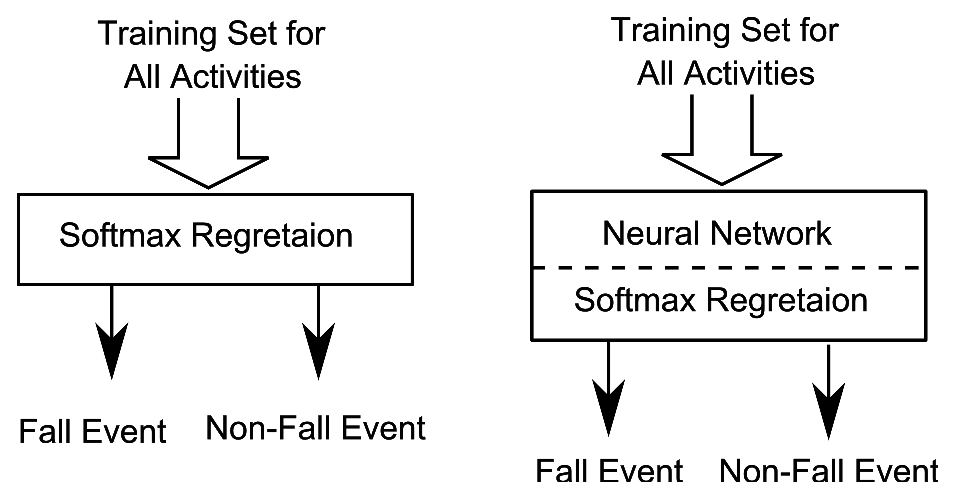
\includegraphics[width=0.98\columnwidth]{figures/SoftmaxLayer1.eps}
	\caption{Layer 1 learning modules. Examples are classified into Fall and Non-Fall events.  The left-side Figure is using Softmax Regression model. The Right-side Figure is a hybrid of Neural Network and Softmax Regression model.}
	\label{fig:SoftmaxLayer1}
\end{figure}

We trained and tested two networks with Softmax regression algorithm. In first case, we trained a one-layer network with 11 binary outputs, one for each fall or non-fall events. In the second case, we trained a two layer softmax regression network. The top layer network was trained with 2 binary outputs to distinguish between fall and non-fall events (see Fig.~\ref{fig:SoftmaxLayer1}). The bottom layer has two sub-networks:  one to identify fall events and has 4 binary outputs, the other to identify non-fall events and has 7 binary outputs. Each sub-network was trained separately. Fig~\ref{fig:SoftmaxLayer2Fall} shows a block diagram of a subnetwork for training and identification of four fall events. For conserving space, we omit diagram for non-fall events. As will be discussed in the next section, none of them identified all events with 100\% accuracy.

\begin{figure}[htbp]
	\centering
		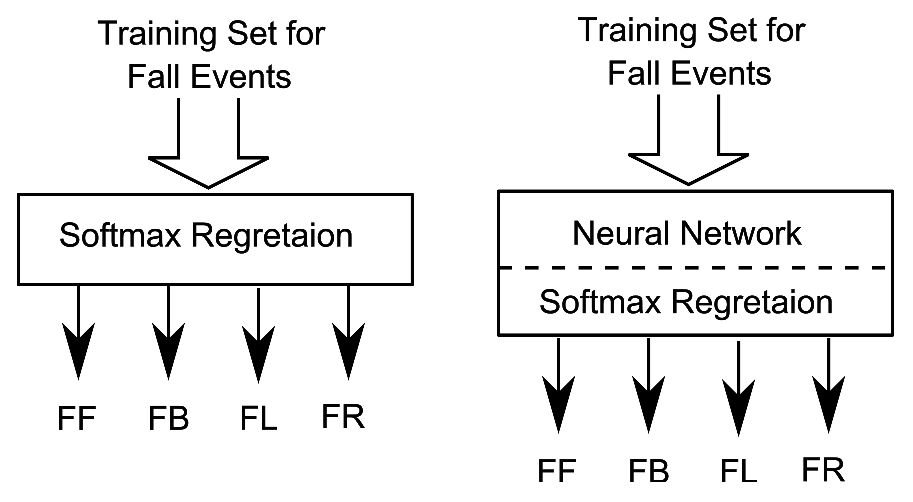
\includegraphics[width=0.98\columnwidth]{figures/SoftmaxLayer2Fall.eps}
	\caption{Layer 2 learning module for four Fall events. The left-side Figure is using Softmax Regression model. The right-side Figure is a hybrid of Neural Network and Softmax Regression }
	\label{fig:SoftmaxLayer2Fall}
\end{figure}

\subsection{Neural Network}
\label{sec:NeuralNetwork}
The second classification network is based on Artificial Neural Network \cite{Bishop06a}. We experimented with both one and two layer networks. Performance of these networks are reported in the next section. None of them identified all evetns with 100\% accuracy.

\subsection{Hybrid Algorithm: Neural Network and Softmax Regreation}
\label{sec:HybridAlgorithmNeuralNetworkAndSoftmaxRegreation}

The hybrid classification network is based on both Artificial Neural Network  and Softmax regression network. Fig.~\ref{fig:SoftmaxLayer1} shows a block diagram of a hybrid network: a single layer of neurons followed by a softmax regression layer.
\par
We have used the prior Softmax activation  and the negative-log likelihood 
functions in the output layer. The hidden layers have used sigmoid activation functions. 
We have also included the bias terms for all hidden layers. The backpropagation algorithm 
has been used to calculate the gradient, while the L-BFGS procedure has been used to 
learn the network parameters. We have independently set each dimension of the sample to 
have zero-mean and unit-variance. We achieved this by first computing the mean of each 
dimension across the training set and subtracting this from each dimension. Then each 
dimension is divided by its standard deviation.       

Similar to Softmax regression networks and Neural networks we experimented  with both single-layer hybrid networks and two-layer hybrid networks. While single-layer network failed to identify all events with 100\% accuracy, the two-layer network successfully identified all event with 100\%. There were no false positives or false negatives.

\section{Online Activity Monitoring and Identification}

In Sections \ref{sec:SemiAutomaticExtractionOfTrainingVectors} and 
\ref{sec:OffLineLearning}, we have discussed the semi-automatic training example 
extraction and the learning of the parameter vectors of the classifiers for the event 
prediction and identification. This process is primarily offline. In operational mode, we 
require that the learned classifiers monitor and identify events online. This section 
provides our setup and methodology.  



\subsection{Monitoring of Event}

For the monitoring of events, we have followed a methodology similar to that of 
Subsection \ref{subsec:preDataCollection}. We have continuously collected the sample data 
to a ring buffer. From a starting marker (initially at the beginning of the ring buffer), 
we have averaged 20 consecutive sample and added that value to a second ring buffer. The 
first ring buffer is incremented by 10 samples, then average the next 20 samples (if the 
data 
is available), and pushed  the average value into the second ring buffer. We have 
continued this process in 
the first ring buffer with 10 samples overlap. In the second ring buffer, we have 
maintained a window of 20 samples. 
In order to compensate for noise, we have used five average values from the window. We 
have 
used the first 20, 18, 16, 14, and 12 average values. These  values are used in the event 
identification. We then incremented the second ring buffer by 10 samples and continued 
the process.  

\begin{figure}[h]
	\centering
		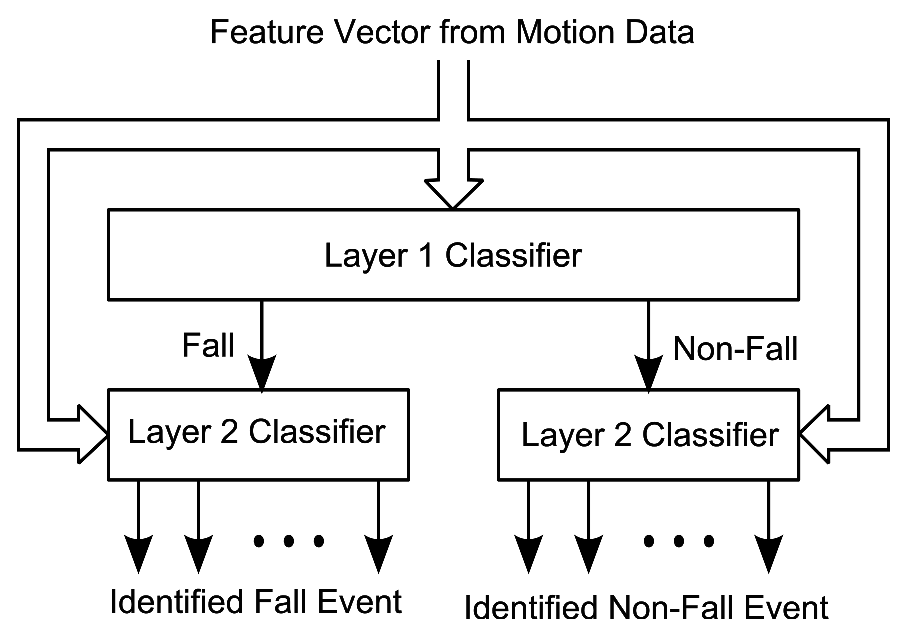
\includegraphics[width=0.48\textwidth]{figures/TrainedIdentificationModule.eps}
	\caption{Block diagram of event identification system. The top layer separates fall events from non-fall events. The bottom layer modules receive the same input data vector as the top layer, but they also get a zero or one input from the upper layer module depending on where the input data vector is classified. The final output is a binary valued vector of 11 components.}
	\label{fig:TrainedIdentificationModule}
\end{figure}


\subsection{Identification of Events}

In order to identify the events, we have used a layered classification network as 
shown in Fig. \ref{fig:TrainedIdentificationModule}. The inputs to the classifiers are 
the 
pre-processed motion data from the previous subsection. In the first layer of our 
classification network (Layer 1), we have used a binary decision classifier that predicts 
whether the current input is a fall or a non-fall. Based on this decision, at the second 
layer of our network (Layer 2), one of the specialized fall event or non-fall activity 
recognition classification network is activated. The decision of this classifier is 
considered as the output of the classification network. In order to compensate for noise, 
we have used the five samples as described in the previous section. We have marked the 
predicted events and if the five samples predict the same outcome, then the network voted 
to that event, otherwise, we have identified an inconclusive event. 



\section{Empirical Evaluation of Proposed Algorithms and Methods}
\label{Evaluation}

%\begin{figure*}[!t]
%\centering
%\subfloat[Human walking 
%forward.]{\label{fig:ha}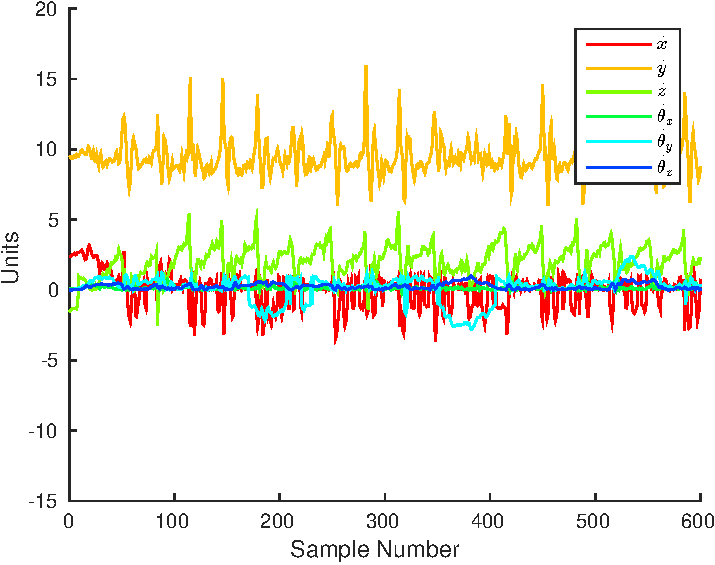
\includegraphics[width=0.25\textwidth]{plots/human_walk2-crop.pdf}}
% 
%\subfloat[Human stand to 
%seat.]{\label{fig:hb}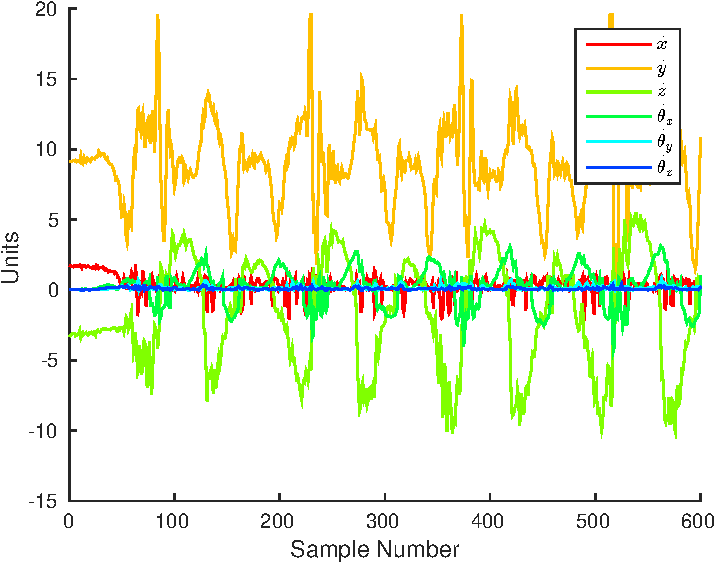
\includegraphics[width=0.25\textwidth]{plots/human_stand2-crop.pdf}}
%%\subfloat[Human stand to 
%%fall.]{\label{fig:hc}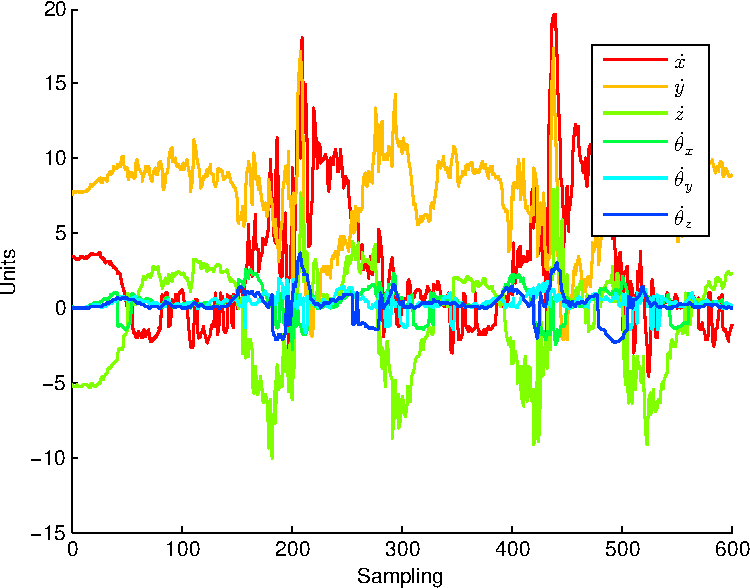
\includegraphics[width=0.32\textwidth]{plots/human_falling-crop.pdf}}
%%\\
%%\subfloat[Robot walk forward.]{\label{fig:ra}\includegraphics[width=0.32\textwidth]
%%{plots/robot_walk_forward-crop.pdf}}
%%\subfloat[Robot walk backward.]{\label{fig:rb}\includegraphics[width=0.32\textwidth]
%%{plots/robot_walk_backward-crop.pdf}}
%%\subfloat[Robot rotate clockwise.]{\label{fig:rc}\includegraphics[width=0.32\textwidth]
%%{plots/robot_rotate_cw-crop.pdf}}
%%\\
%\subfloat[Robot fallen forward.]{\label{fig:rd}\includegraphics[width=0.25\textwidth]
%{plots/robot_fallen_forward2-crop.pdf}} 
%\subfloat[Robot fallen backward.]{\label{fig:re}\includegraphics[width=0.25\textwidth]
%{plots/robot_fallen_backward2-crop.pdf}}
%%\subfloat[Robot fallen right.]{\label{fig:rf}\includegraphics[width=0.32\textwidth]
%%{plots/robot_fallen_right-crop.pdf}}
%
%\caption{Figures (a--b) shows 3-axis accelerometer and 3-axis gyroscope graph for human 
%motions 
%walking forward and stand to seat. Figures (c--d) shows 3-axis accelerometer and 3-axis 
%gyroscope 
%graph for robot's fallen forward and backward motions.}
% \label{fig:anotation-human-robot} 
%\end{figure*}
%% Figures (d)-(f) shows 3-axis accelerometer and 3-axis gyroscope graph for robot's walk 
%%motion. 

TODO: put the numbers into the description provided in the previous sections. 

\subsection{Results}

\begin{table}[!b]
\caption{fixme: Softmax: 94.4}
\resizebox{\columnwidth}{!}
{
\begin{tabular}{|c|c|c|c|c|c|c|c|c|c|c|c|}
\hline 
& \textbf{FF} & \textbf{FB}  & \textbf{FL} & \textbf{FR} &  \textbf{WF} & 
\textbf{WB} & \textbf{WL} & \textbf{WR} & \textbf{MR} & 
\textbf{RC} & \textbf{RA} \\ \hline
\textbf{FF} & 66.7 &  0 &  0 &  0 &  0 &  16.7 &  0 &  0 &  16.7 &  0 &  0 \\ \hline
\textbf{FB} & 0 &  100 &  0 &  0 &  0 &  0 &  0 &  0 &  0 &  0 &  0 \\ \hline
\textbf{FL} & 0 &  0 &  100 &  0 &  0 &  0 &  0 &  0 &  0 &  0 &  0 \\ \hline
\textbf{FR} & 0 &  0 &  0 &  100 &  0 &  0 &  0 &  0 &  0 &  0 &  0 \\ \hline
\textbf{WF} & 0 &  0 &  0 &  0 &  87.5 &  0 &  0 &  12.5 &  0 &  0 &  0 \\ \hline
\textbf{WB} & 0 &  0 &  0 &  0 &  0 &  100 &  0 &  0 &  0 &  0 &  0 \\ \hline
\textbf{WL} & 0 &  0 &  0 &  0 &  0 &  0 &  100 &  0 &  0 &  0 &  0 \\ \hline
\textbf{WR} & 0 &  0 &  0 &  0 &  0 &  0 &  12.5 &  87.5 &  0 &  0 &  0 \\ \hline
\textbf{MR} & 0 &  0 &  0 &  0 &  0 &  0 &  0 &  0 &  100 &  0 &  0 \\ \hline
\textbf{RC} & 0 &  0 &  0 &  0 &  0 &  0 &  0 &  0 &  0 &  100 &  0 \\ \hline
\textbf{RA} & 0 &  0 &  0 &  0 &  0 &  0 &  0 &  0 &  0 &  0 &  100 \\ \hline
\end{tabular}
}
\end{table}

\begin{table}
\caption{fixme: Neural network: 95.8}
\resizebox{\columnwidth}{!}
{
\begin{tabular}{|c|c|c|c|c|c|c|c|c|c|c|c|}
\hline 
& \textbf{FF} & \textbf{FB}  & \textbf{FL} & \textbf{FR} &  \textbf{WF} & 
\textbf{WB} & \textbf{WL} & \textbf{WR} & \textbf{MR} & 
\textbf{RC} & \textbf{RA} \\ \hline
\textbf{FF} & 66.7 &  0 &  0 &  0 &  0 &  0 &  16.7 &  0 &  16.7 &  0 &  0 \\ \hline
\textbf{FB} & 0 &  100 &  0 &  0 &  0 &  0 &  0 &  0 &  0 &  0 &  0 \\ \hline
\textbf{FL} & 0 &  0 &  100 &  0 &  0 &  0 &  0 &  0 &  0 &  0 &  0 \\ \hline
\textbf{FR} & 0 &  0 &  0 &  100 &  0 &  0 &  0 &  0 &  0 &  0 &  0 \\ \hline
\textbf{WF} & 0 &  0 &  0 &  0 &  100 &  0 &  0 &  0 &  0 &  0 &  0 \\ \hline
\textbf{WB} & 0 &  0 &  0 &  0 &  0 &  100 &  0 &  0 &  0 &  0 &  0 \\ \hline
\textbf{WL} & 0 &  0 &  0 &  0 &  0 &  0 &  100 &  0 &  0 &  0 &  0 \\ \hline
\textbf{WR} & 0 &  0 &  0 &  0 &  0 &  0 &  12.5 &  87.5 &  0 &  0 &  0 \\ \hline
\textbf{MR} & 0 &  0 &  0 &  0 &  0 &  0 &  0 &  0 &  100 &  0 &  0 \\ \hline
\textbf{RC} & 0 &  0 &  0 &  0 &  0 &  0 &  0 &  0 &  0 &  100 &  0 \\ \hline
\textbf{RA} & 0 &  0 &  0 &  0 &  0 &  0 &  0 &  0 &  0 &  0 &  100 \\ \hline
\end{tabular}
}
\end{table}

\begin{table}
\caption{fixme: Softmax L1: 87.17, fixme: Neural network L1: 100}
\resizebox{\columnwidth}{!}
{
\begin{tabular}{|c|c|c||c|c|}
\hline
& \multicolumn{2}{c||}{\bf Softmax L1: 87.2} & \multicolumn{2}{c|}{\bf Neural L1: 
100} \\ \hline
& \textbf{Fall Event} & \textbf{Non-Fall Event}  & \textbf{Fall Event} & \textbf{Non-Fall 
Event} \\ \hline
\textbf{Fall Event} & 85.7 &  14.3  & 100 &  0 \\ \hline
\textbf{Non-Fall Event} & 12.7 &  87.3 & 0 &  100 \\ \hline
\end{tabular}
}
\end{table}


\begin{table}
\caption{fixme: Softmax: L2\_true: 100, Neural network: L2\_true: 100}
%\resizebox{\columnwidth}{!}
{
\begin{tabular}{|c|c|c|c|c||c|c|c|c|}
\hline 
& \multicolumn{4}{c||}{\bf Softmax: L2 Fall Event: 100} & \multicolumn{4}{c|}{\bf Neural 
L2 Fall Event: 100} \\ \hline
& \textbf{FF} & \textbf{FB}  & \textbf{FL} & \textbf{FR} & \textbf{FF} & \textbf{FB}  & 
\textbf{FL} & \textbf{FR} \\ \hline
\textbf{FF} & 100 &  0 &  0 &  0  & 100 &  0 &  0 &  0\\ \hline
\textbf{FB} & 0 &  100 &  0 &  0  & 0 &  100 &  0 &  0\\ \hline
\textbf{FL} & 0 &  0 &  100 &  0  & 0 &  0 &  100 &  0\\ \hline
\textbf{FR} & 0 &  0 &  0 &  100  & 0 &  0 &  0 &  100 \\ \hline
\end{tabular}
}
\end{table}

\begin{table}
\caption{fixme: Softmax: L2\_negg: 100}
%\resizebox{\columnwidth}{!}
{
\begin{tabular}{|c|c|c|c|c|c|c|c|}
\hline 
 & \textbf{WF} & \textbf{WB} & \textbf{WL} & \textbf{WR} & \textbf{MR} & 
\textbf{RC} & \textbf{RA} \\ \hline    
\textbf{WF} & 100 &  0 &  0 &  0 &  0 &  0 &  0 \\ \hline
\textbf{WB} & 0 &  100 &  0 &  0 &  0 &  0 &  0 \\ \hline
\textbf{WL} & 0 &  0 &  100 &  0 &  0 &  0 &  0 \\ \hline
\textbf{WR} & 0 &  0 &  0 &  100 &  0 &  0 &  0 \\ \hline
\textbf{MR} & 0 &  0 &  0 &  0 &  100 &  0 &  0 \\ \hline
\textbf{RC} & 0 &  0 &  0 &  0 &  0 &  100 &  0 \\ \hline
\textbf{RA} & 0 &  0 &  0 &  0 &  0 &  0 &  100 \\ \hline
\end{tabular}
}
\end{table}

\begin{table}
\caption{ixme: Neural network: L2\_negg: 100}
%\resizebox{\columnwidth}{!}
{
\begin{tabular}{|c|c|c|c|c|c|c|c|}
\hline 
 & \textbf{WF} & \textbf{WB} & \textbf{WL} & \textbf{WR} & \textbf{MR} & 
\textbf{RC} & \textbf{RA} \\ \hline 
\textbf{WF} & 100 &  0 &  0 &  0 &  0 &  0 &  0 \\ \hline
\textbf{WB} & 0 &  100 &  0 &  0 &  0 &  0 &  0 \\ \hline
\textbf{WL} & 0 &  0 &  100 &  0 &  0 &  0 &  0 \\ \hline
\textbf{WR} & 0 &  0 &  0 &  100 &  0 &  0 &  0 \\ \hline
\textbf{MR} & 0 &  0 &  0 &  0 &  100 &  0 &  0 \\ \hline
\textbf{RC} & 0 &  0 &  0 &  0 &  0 &  100 &  0 \\ \hline
\textbf{RA} & 0 &  0 &  0 &  0 &  0 &  0 &  100 \\ \hline
\end{tabular}
}
\end{table}



We have conducted our experiments on detecting eight regular movement activities and four fall events on 
%able-bodied 
humans. The list of these activities and fall events are shown in Table~\ref{tab:human-logistic-class}. For humanoid robots (NAO robots) we evaluated all these activities and fall events, except stand-to-sit activity. 
 A wireless 9-axis  motion sensing device was attached to the back of the subjects as shown in Fig.~\ref{fig:framework}, and a wireless data collecting device was connected to a computer. These two devices formed a WSN. While each subject was performing each of the prescribed activities, and fall events data was logged in the computer for leaning and performance evaluation.
\par
The motion data included 3-axis accelerometer readings, 3-axis gyroscope readings, and 3-axis magnetometer readings. These datasets were used to calculate
the quaternion rotation axis of the device, and Euler angles roll, pitch, and yaw. We have used the Direction Cosine Matrix (DCM) algorithm for calculating Euler angles. 
\par
The rest of the  section reports our data collection, data processing, learning, 
and prediction results.


%\subsubsection{Activity Annotation:} The annotation for different human and robot motion 
%activities 
%are shown in 
%Figure {~\ref{fig:anotation-human-robot}}. 
%Accelerometer and gyroscope's $x$, $y$ and $z$ axis are shown for different motions. We 
%can observe 
%that transition from a routine motion activity to a fall event 
%takes between 180 to 250 ms. Figure{~\ref{fig:anotation-human-robot}} (a--b) shows the 
%activity annotations for human motions (walking forward and sitting down). 
%Figure {~\ref{fig:anotation-human-robot}}
%(c--d) shows activity annotations for the NAO robot. The following section provides the 
%evaluation 
%matrices of our experiments. 


%\section{Evaluation Results}
%%\subsection{Learning Algorithms}
%We have structured this section in a way that we discuss feature extraction, data 
%processing, 
%machine learning, and experimental results for both the human and robotic experiments. 
%We have 
%tested our hypotheses using  {\em Regularized Logistic Regression} (LLR) and {\em 
%Support 
%Vector Machine} (SVM) algorithms. We have used a randomly generated 80\%--20\% partition 
%for 
%training and cross-validation on our learning dataset. We have used an independent test 
%set to 
%report our results. We have used standard parameter sweeping techniques to find the 
%classifier 
%parameters that provide the optimal trade-off between the bias and the variance, while 
%precision, 
%recall, and F$_1$-scores have been used to obtain the optimal value. 
%
%\subsection{Feature Extraction}
%
%We  have configured the motion sensor to sample at every  $20ms$, which is equivalent to 
%50$Hz$ 
%sampling rate. In order to 
%identify activities: \begin{inparaenum}[1)] \item we have used a window size of $400ms$ 
%(20 
%samples); and \item we have allowed 10 samples ($200ms$) to overlap between windows. 
%\end{inparaenum} The selection of the window size is based on the observation that 
%transition from routine  activities to a fall event 
%takes between $180-250ms$. Thus, a window size of $400ms$ will include both fall event 
%and 
%non-fall event data for classification. For each window, we have calculated the running 
%average of 
%all 9-axis values. This has produced nine values per window, which has been used as 
%features. We 
%also added a bias term to provide additional capacity for the learning algorithms. The  
%accelerometer readings are in  meter per square second ($m/s^2$), gyroscope readings are 
%in 3-axis in radian per square second ($rads/s^2$), and the magnetometer readings are  
%in 
%Tesla ($T$). 
%
%As a preprocessing step, the features, except the bias, have been subjected to feature 
%standardization. We have independently set each dimension of the sample  to have 
%zero-mean and 
%unit-variance. We achieved this by first computing the mean of each dimension across the 
%dataset and 
%subtracting this from each dimension. Then each dimension is divided by its standard 
%deviation.
 

\subsection{Experiments with a Human}

%We have attached the sensors on the mid-back of the human body as shown in Figure \ref{fig:fb} for 
%collecting our datasets. 

We have defined a protocol that collects data for seven normal activities and four falling events 
as 
shown in Table \ref{tab:human-logistic-class}. The normal activities include walking 
(forward, backward, left, and right), marching, and rotating (left and right). Falling  (forward, 
backward, left, and right) has been considered as an abnormal event.  The same protocol has also 
been applied to the 
humanoid robot (Table \ref{tab:robot-logistic-class}), because  motion characteristics of the human and the 
robot are very similar. In addition, we 
have  defined an extended activity, stand to seat, on the human. Therefore, we have conducted 
twelve motions in total on the human subject.  Example plots for 
\begin{inparaenum}[($i$)] \item walking forward; and \item from standing to sitting 
down  \end{inparaenum}  are shown in Figures \ref{fig:ha} and \ref{fig:hb} respectively. 


 



\subsubsection{Results:} Table \ref{tab:human-logistic-class} shows the final results for 
LLR classification, where, true positive, true negative, false positive, and false negative are 
abbreviated with TP, TN, FP, and FN respectively. For walking forward on an average, the accuracy is 91\%, 
similarly, for falling forward and marching the accuracies are 94\% and 91\% on an 
average, respectively. We found comparatively low accuracy in walking backward and falling backward. Rotation has accuracy on an average more than 90\%. We also observed that detection of the walking activity is less than other 
activities that we experimented with.  

%\begin{figure*}[!t]
  %\centering
  %\subfloat[Marching in place.]{\label{fig:tsnedataset_1}\includegraphics[width=0.25\textwidth]
       %{figures/plot1-crop}} 
  %\subfloat[Walking backward.]{\label{fig:tsnedataset_9}\includegraphics[width=0.25\textwidth]
       %{figures/plot5-crop}}
%%  \subfloat[Rotating clockwise.]{\label{fig:tsnedataset_7}\includegraphics[width=0.25\textwidth]
%%       {plot2-crop}}
%%  \subfloat[Left side-way walk.]{\label{fig:tsnedataset_10}\includegraphics[width=0.25\textwidth]
%%       {plot6-crop}}
%%       \\
  %\subfloat[Falling forward.]{\label{fig:tsnedataset_11}\includegraphics[width=0.25\textwidth]
       %{figures/plot1_fallen-crop}}
  %\subfloat[Falling backward.]{\label{fig:tsnedataset_12}\includegraphics[width=0.25\textwidth]
       %{figures/plot2_fallen-crop}}
%%  \subfloat[Falling to left side.]{\label{fig:tsnedataset_13}\includegraphics[width=0.25\textwidth]
%%       {plot3_fallen-crop}}
%%  \subfloat[Falling to right
%%side.]{\label{fig:tsnedataset_14}\includegraphics[width=0.25\textwidth]
%%       {plot4_fallen-crop}}      
  %\caption{Figures (a--b) show the roll and pitch angles (raw and filtered) for normal 
%behaviors marching in place and walking backward. Figures (c--d) show the raw and filtered roll 
%and pitch angles for fallen forward and backwards states of NAO humanoid robot.}
  %\label{fig:normalFallenBehavior}
%
%\end{figure*}

The results for SVM classifier is summarized in Table \ref{tab:human-svm-class}. On an average, 
accuracy for each type of activity is higher than LLR classifier with on an average 96\% for 
walking, 95\% for marching, and 96\% for falling forward. Both type of rotations have little higher accuracy over LLR. As a consequence, SVM classifier has less false positives and false negative compared to LLR.  Our experiments reveal that the SVM classifier performs better than the logistic regression classifier. However, due to memory and 
computational restrictions on the embedded devices, we have found that the logistic 
regression classifier is a better choice.  Our feature vector consists of the mean normalized sensor 
reading and a bias term. We plan to combine and prune features to improve the classification 
accuracy for future work.  




\section{Conclusions and Future Work}

%It is known that while humans and biped humanoid robots perform normal activities such as jogging, 
%running and so on, an abnormal event such as a fall may occur. These events may cause injuries 
 %to the humans or robots. 
%  In order to avoid 
%  damages to biped humanoid robots, machine learning can be used to predict potential falls before 
%  such events occur. 
Falling events could cause damage to both humans and robots.  Using prediction information, 
corrective measures can be engaged to avoid 
 many fall events. Similarly, for humans, after  a fall is identified, rescue services 
 can be called upon. We have reported a wireless sensing device that have assembled using 
off-the-shelf hardware components. Using two devices, we have created a sensor network for 
collecting motion data from humans and biped humanoid robots. The sensing devices were connected to 
the back of the subjects and the data collecting device was connected to a laptop which archived 
the data. We have used two machine learning algorithms and thresholding methods to 
identify both normal and abnormal activities within 91\%--100\% accuracy. Comparing the encouraging 
experimental results we achieved, our future work will be to use multiple sensing devices to create 
a sensor network to detect complex activities with higher sampling rates.  

\bibliographystyle{plain}
\bibliography{references,fallRisk}

%\end{sloppy}
\end{document}
